%%%%%%%%%%%%%%%%%%%%%%%%%%%%%%%%%%%%%%%%%%%%%%%%%%%%%%%%%
%%   $RCSfile: hpsg04.tex,v $
%%  $Revision: 1.1 $
%%      $Date: 2004/08/11 09:53:01 $
%%     Author: Stefan Mueller (CL Uni Bremen)
%%    Purpose: 
%%   Language: LaTeX
%%%%%%%%%%%%%%%%%%%%%%%%%%%%%%%%%%%%%%%%%%%%%%%%%%%%%%%%%
%%
%% $Log: hpsg04.tex,v $
%% Revision 1.1  2004/08/11 09:53:01  stefan
%% *** empty log message ***
%%
%% Revision 1.1  2003/10/12 13:42:57  stefan
%% Initial revision
%%
%%%%%%%%%%%%%%%%%%%%%%%%%%%%%%%%%%%%%%%%%%%%%%%%%%%%%%%%%

\documentclass[11pt,a4paper,fleqn]{article}
\usepackage{times}
\thispagestyle{empty}



\usepackage[T1]{fontenc}   % Silbentrennung

\usepackage{8bit}

\usepackage[bookmarks=true,bookmarksopen=true,%
breaklinks=true,%
draft=false,colorlinks=false,plainpages=false,hyperfootnotes=false,%
linkcolor=black,%
pagecolor=black,%
pdfauthor={Stefan M�ller (Editor)},%
pdftitle={Proceedings of the HPSG06 Conference},%
pdfkeywords={HPSG}%,
pdftex=true%
%ps2pdf=true  %ohne diesen Treiber geht der Zeilenumbruch in URLs
]{hyperref}% for pdf files

\usepackage{pdfpages}


\hypersetup{colorlinks=false, pdfborder={0 0 0}}

\begin{document}

\begin{center}
{\Large
                   Proceedings of the HPSG07 Conference\\[\baselineskip]

Stanford Department of Linguistics and CSLI's LinGO Lab\\[\baselineskip]

                        Stefan M{\"u}ller (Editor)\\[\baselineskip]

                                2007\\[\baselineskip]

                          CSLI Publications\\[\baselineskip]

              http://csli-publications.stanford.edu/
}
\end{center}
\newpage
\tableofcontents

\newpage

\section{Editor's Note}

The 14th International Conference on Head-Driven Phrase Structure Grammar (2007) was held in Stanford
and organized by the Stanford Department of Linguistics and CSLI's LinGO Lab.

The conference featured 2 invited talks and 18 papers
selected by the program committee 
(Doug Arnold,      
Emily M. Bender,	
Olivier Bonami,	
Ann Copestake,	
Berthold Crysmann,
Dan Flickinger,	
Tibor Kiss,	
Jong-Bok Kim,	
Robert Levine,	
Tsuneko Nakazawa,
Stefan M�ller (chair),
Gerald Penn,	
Adam Przepiorkowski,
Ivan Sag,	
Jesse Tseng,	
Detmar Meurers,	  
Frank Van Eynde,
Gertjan van Noord,
Gert Webelhuth,	
Stephen Wechsler).

A workshop about \emph{Constructions and Grammatical Theory}
was attached to the conference. It featured three invited talks
and 4 papers, selected by the program committee.

In total there were 38 submissions to the main conference and to the
workshop. 
We want to thank the respective program committee for putting this nice program together.



Thanks go to Ivan Sag, who was in charge of local arrangements.


As in the past years the contributions to the conference proceedings are based on the five page abstract
that was reviewed by the respective program committees, but there is no additional reviewing of the
longer contribution to the proceedings.
To ensure easy access and fast publication we have chosen an electronic format.


The proceedings include all the papers except those by Adele Goldberg and Christopher Manning.



\newpage
\part{Contributions to the Main Conference}



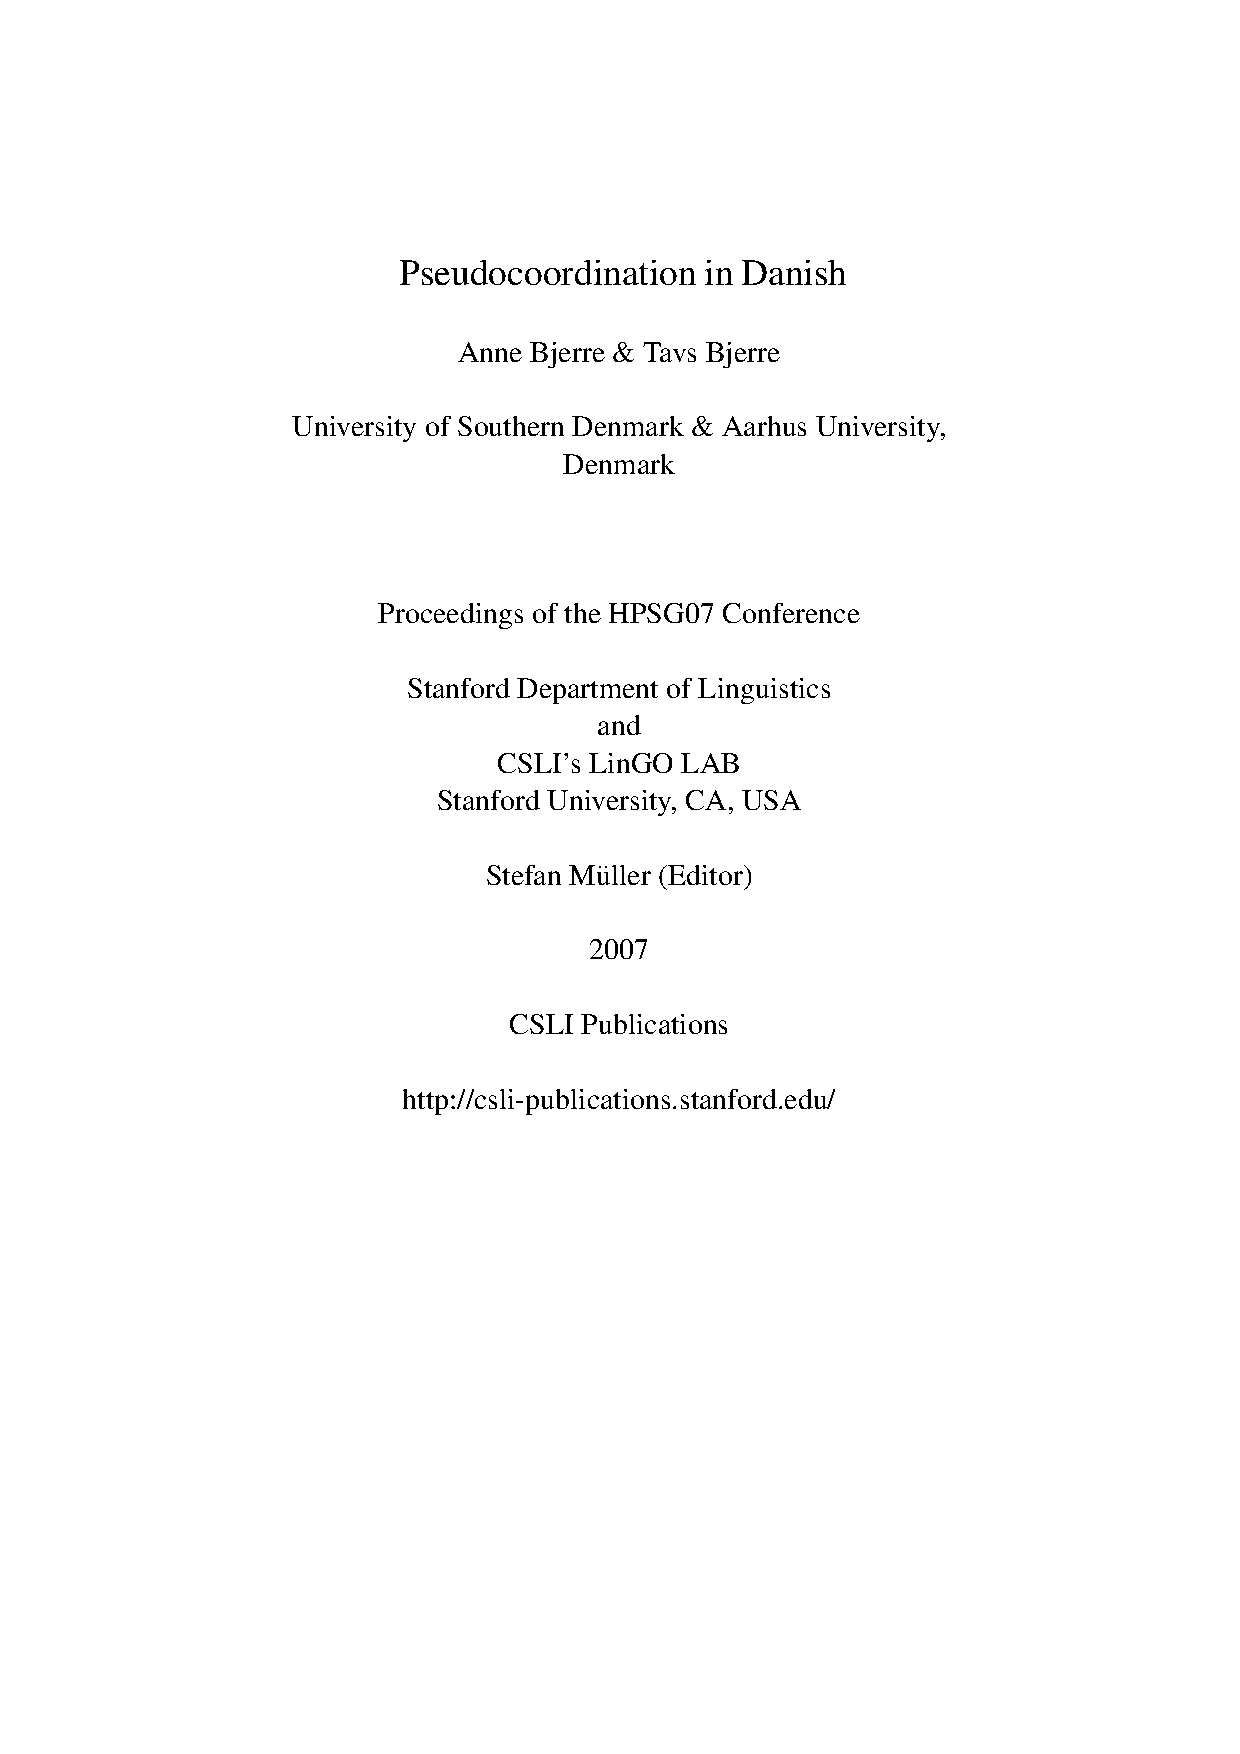
\includepdf[pages=-,pagecommand=\thispagestyle{plain},
            addtotoc={1,section,1,
            {Anne Bjerre and Tavs Bjerre: Pseudocoordination in Danish},
             bjerre}]{bjerre-bjerre.pdf}

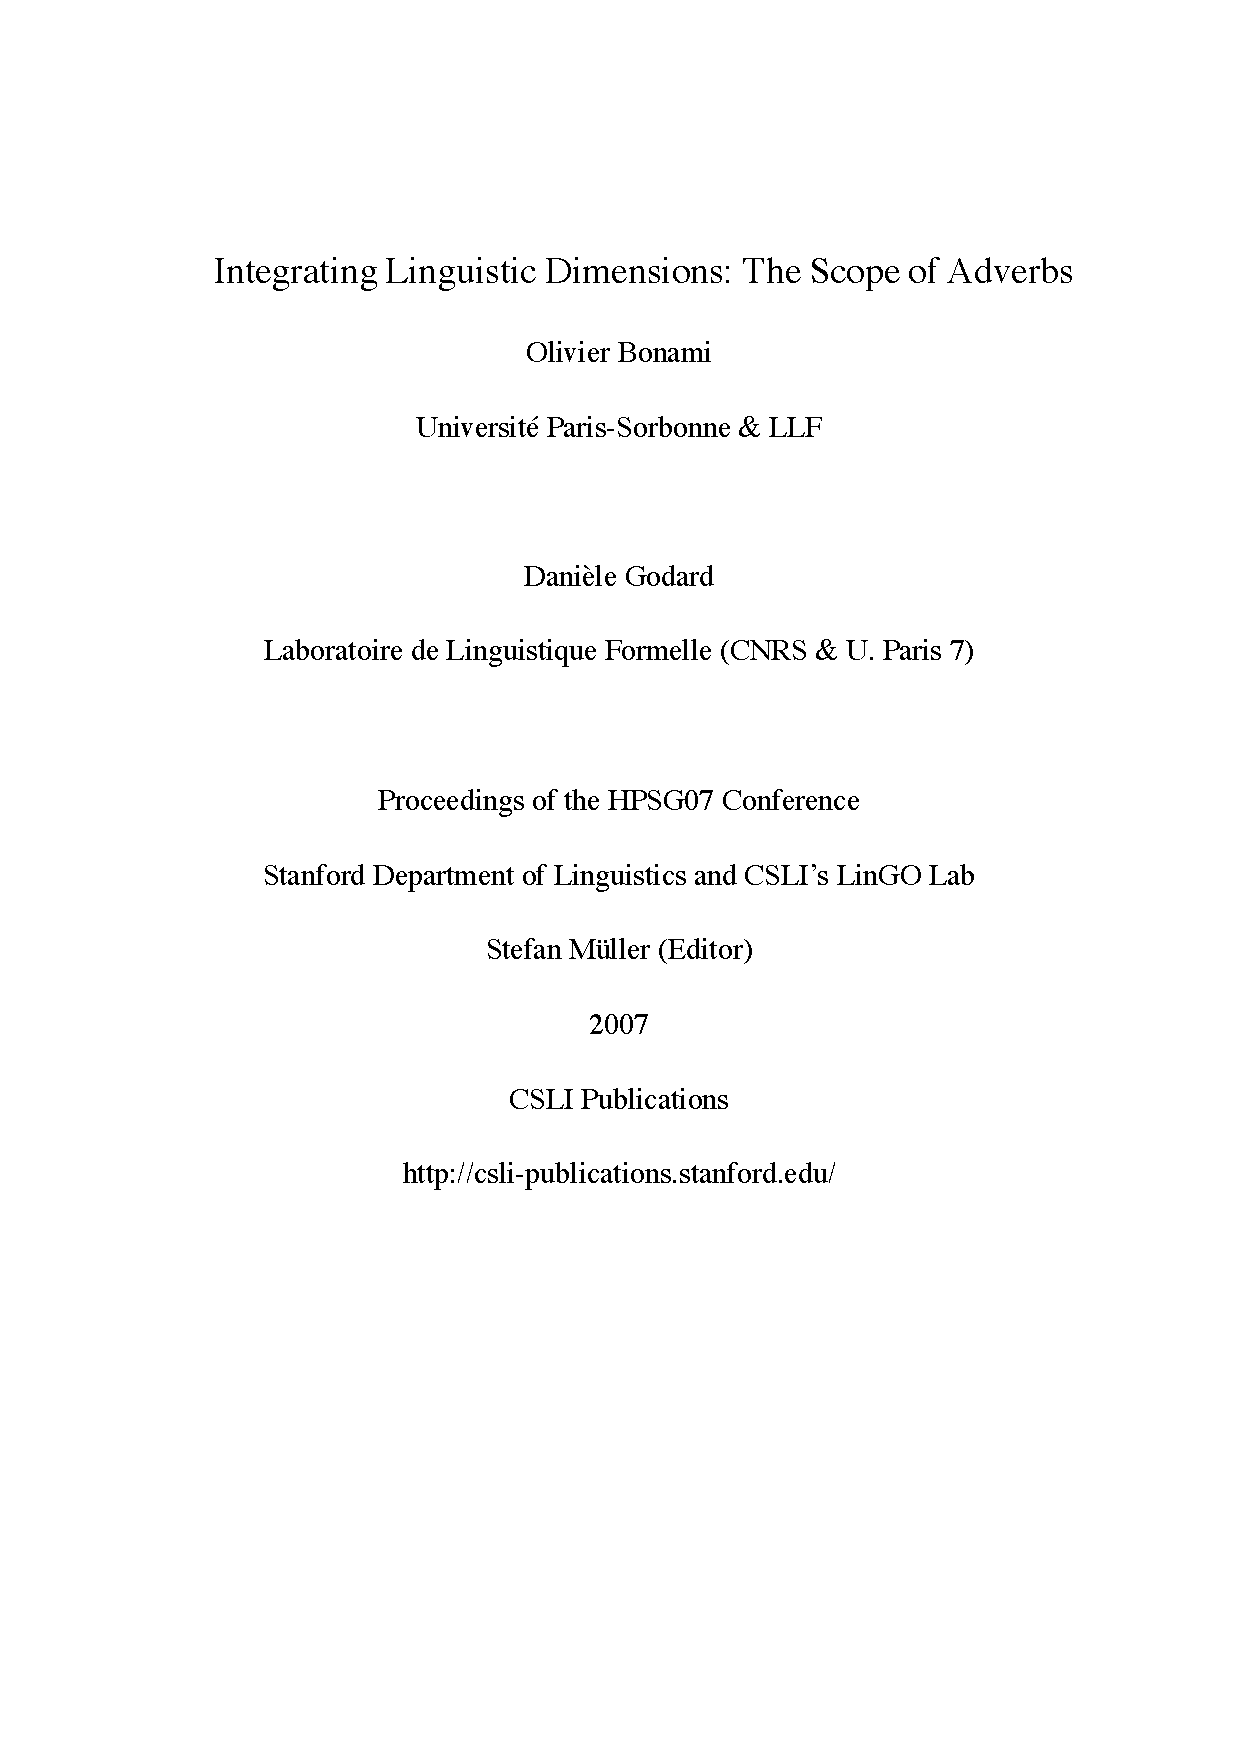
\includepdf[pages=-,pagecommand=\thispagestyle{plain},
            addtotoc={1,section,1,
            {Olivier Bonami and Dani�le Godard: Integrating Linguistic Dimensions: The Scope of Adverbs},
             bg}]{bonami-godard.pdf}


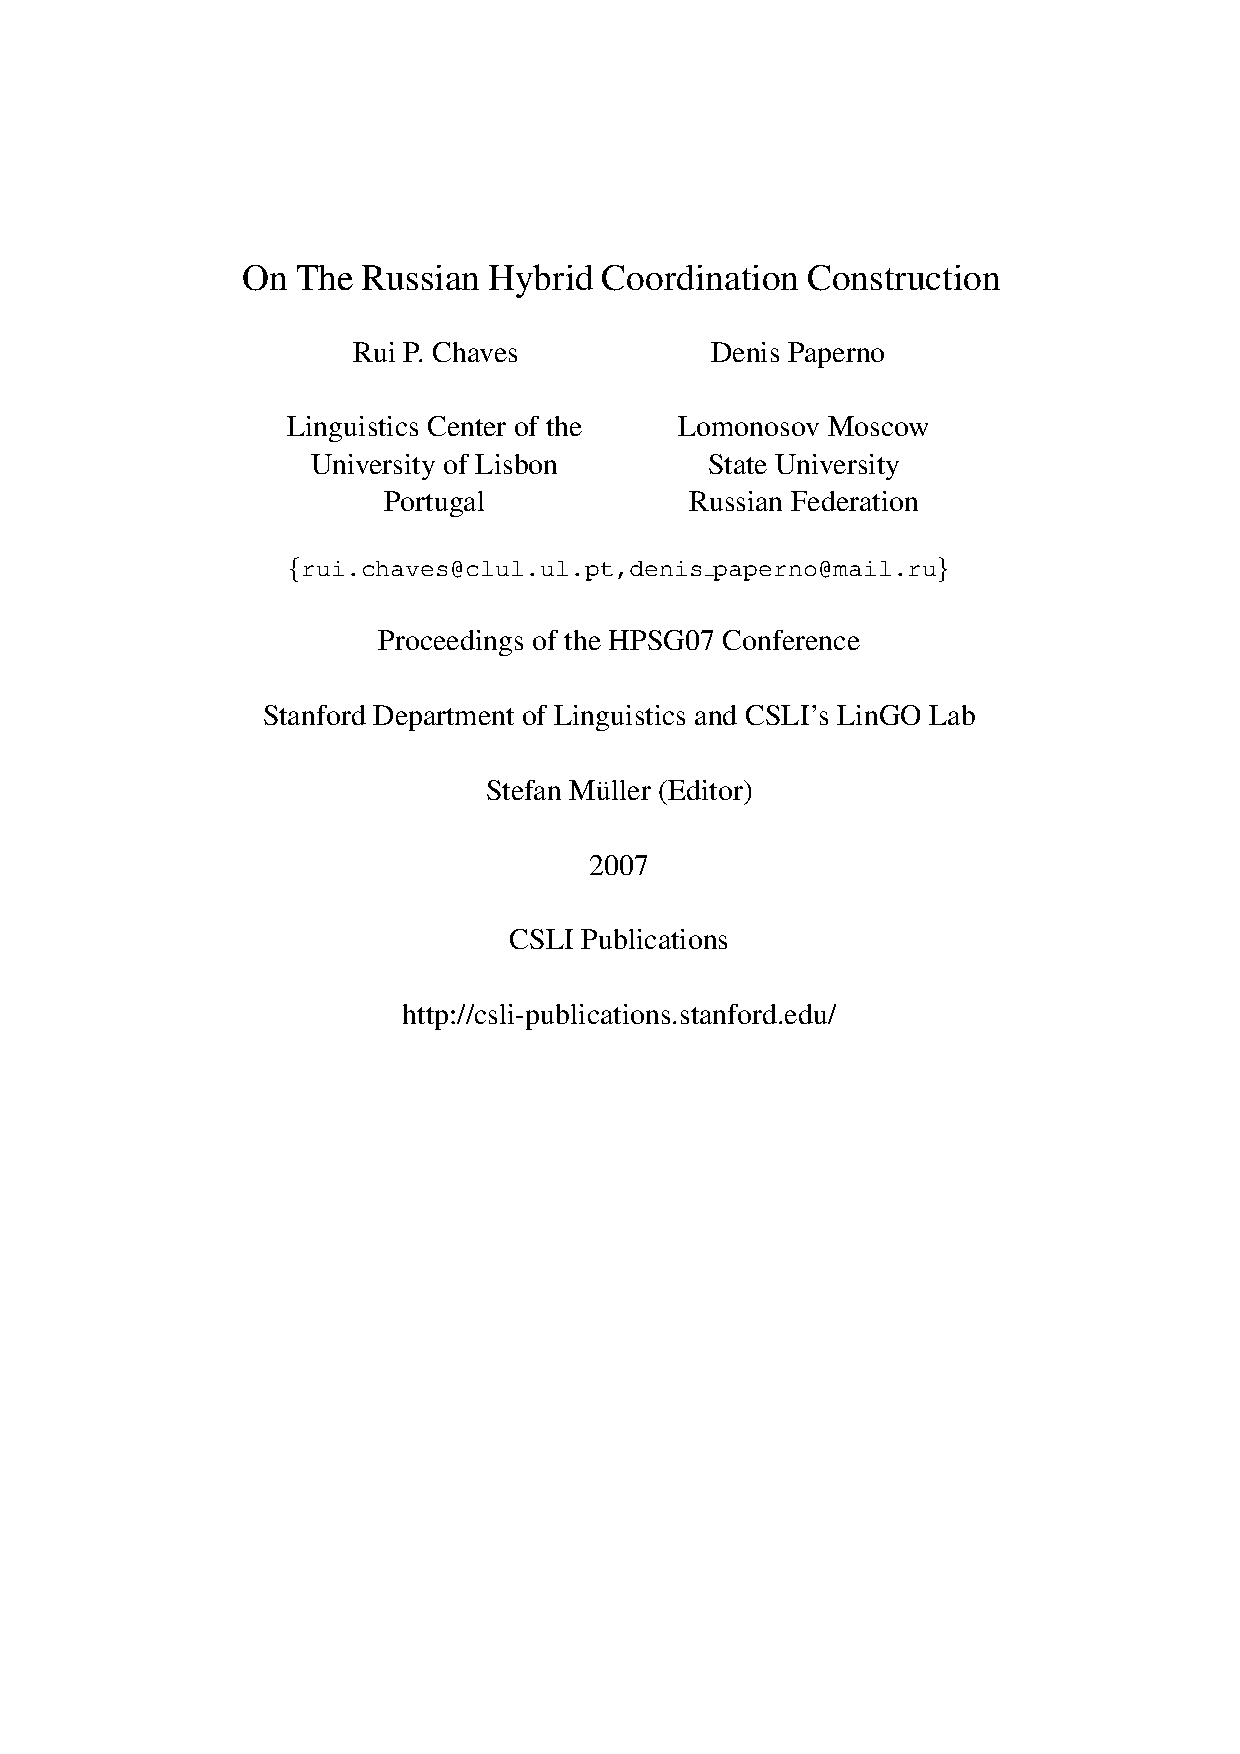
\includepdf[pages=-,pagecommand=\thispagestyle{plain},
            addtotoc={1,section,1,
            {Rui P. Chaves and Denis Paperno: On The Russian Hybrid Coordination Construction},
             chaves}]{chaves-paperno.pdf}

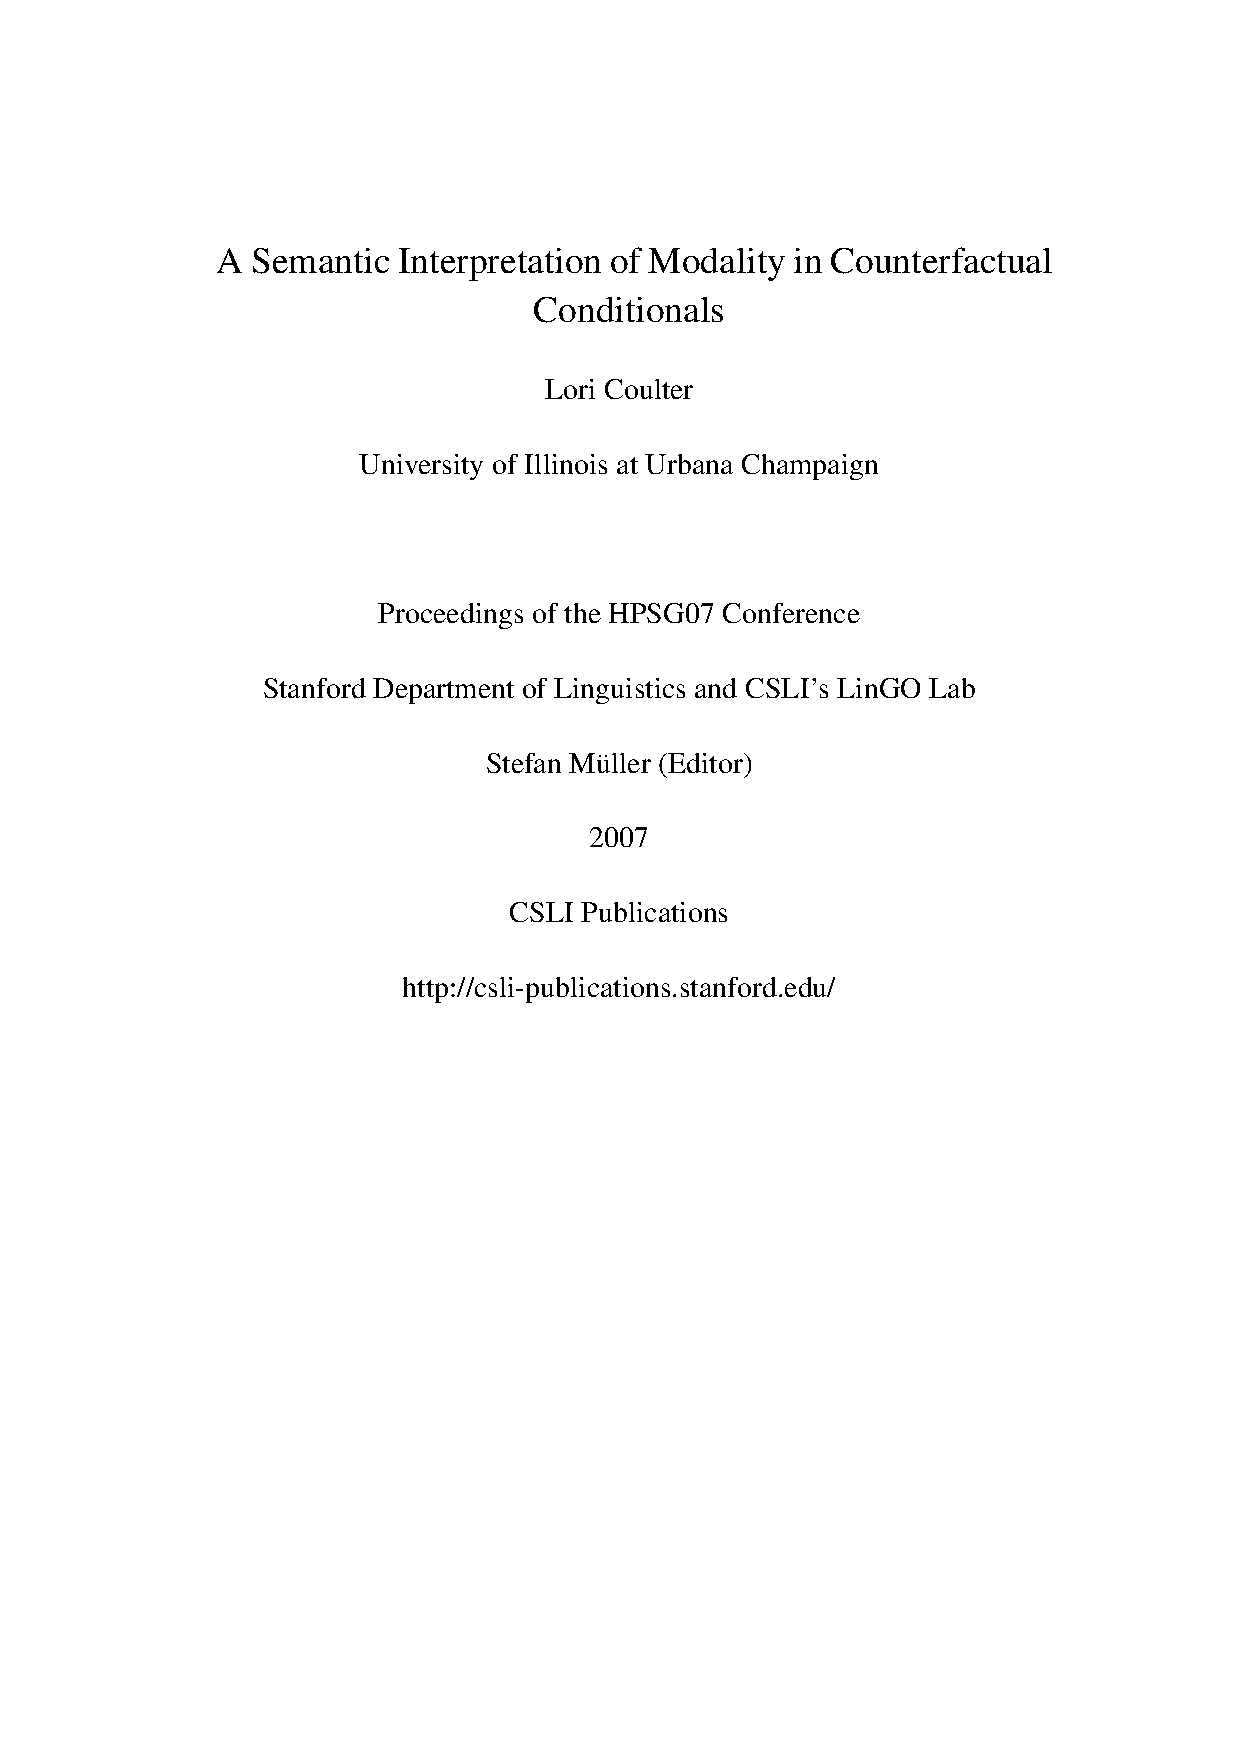
\includepdf[pages=-,pagecommand=\thispagestyle{plain},
            addtotoc={1,section,1,
            {Lori Coulter: A Semantic Interpretation of Modality in Counterfactual Conditionals},
             coulter}]{coulter.pdf}


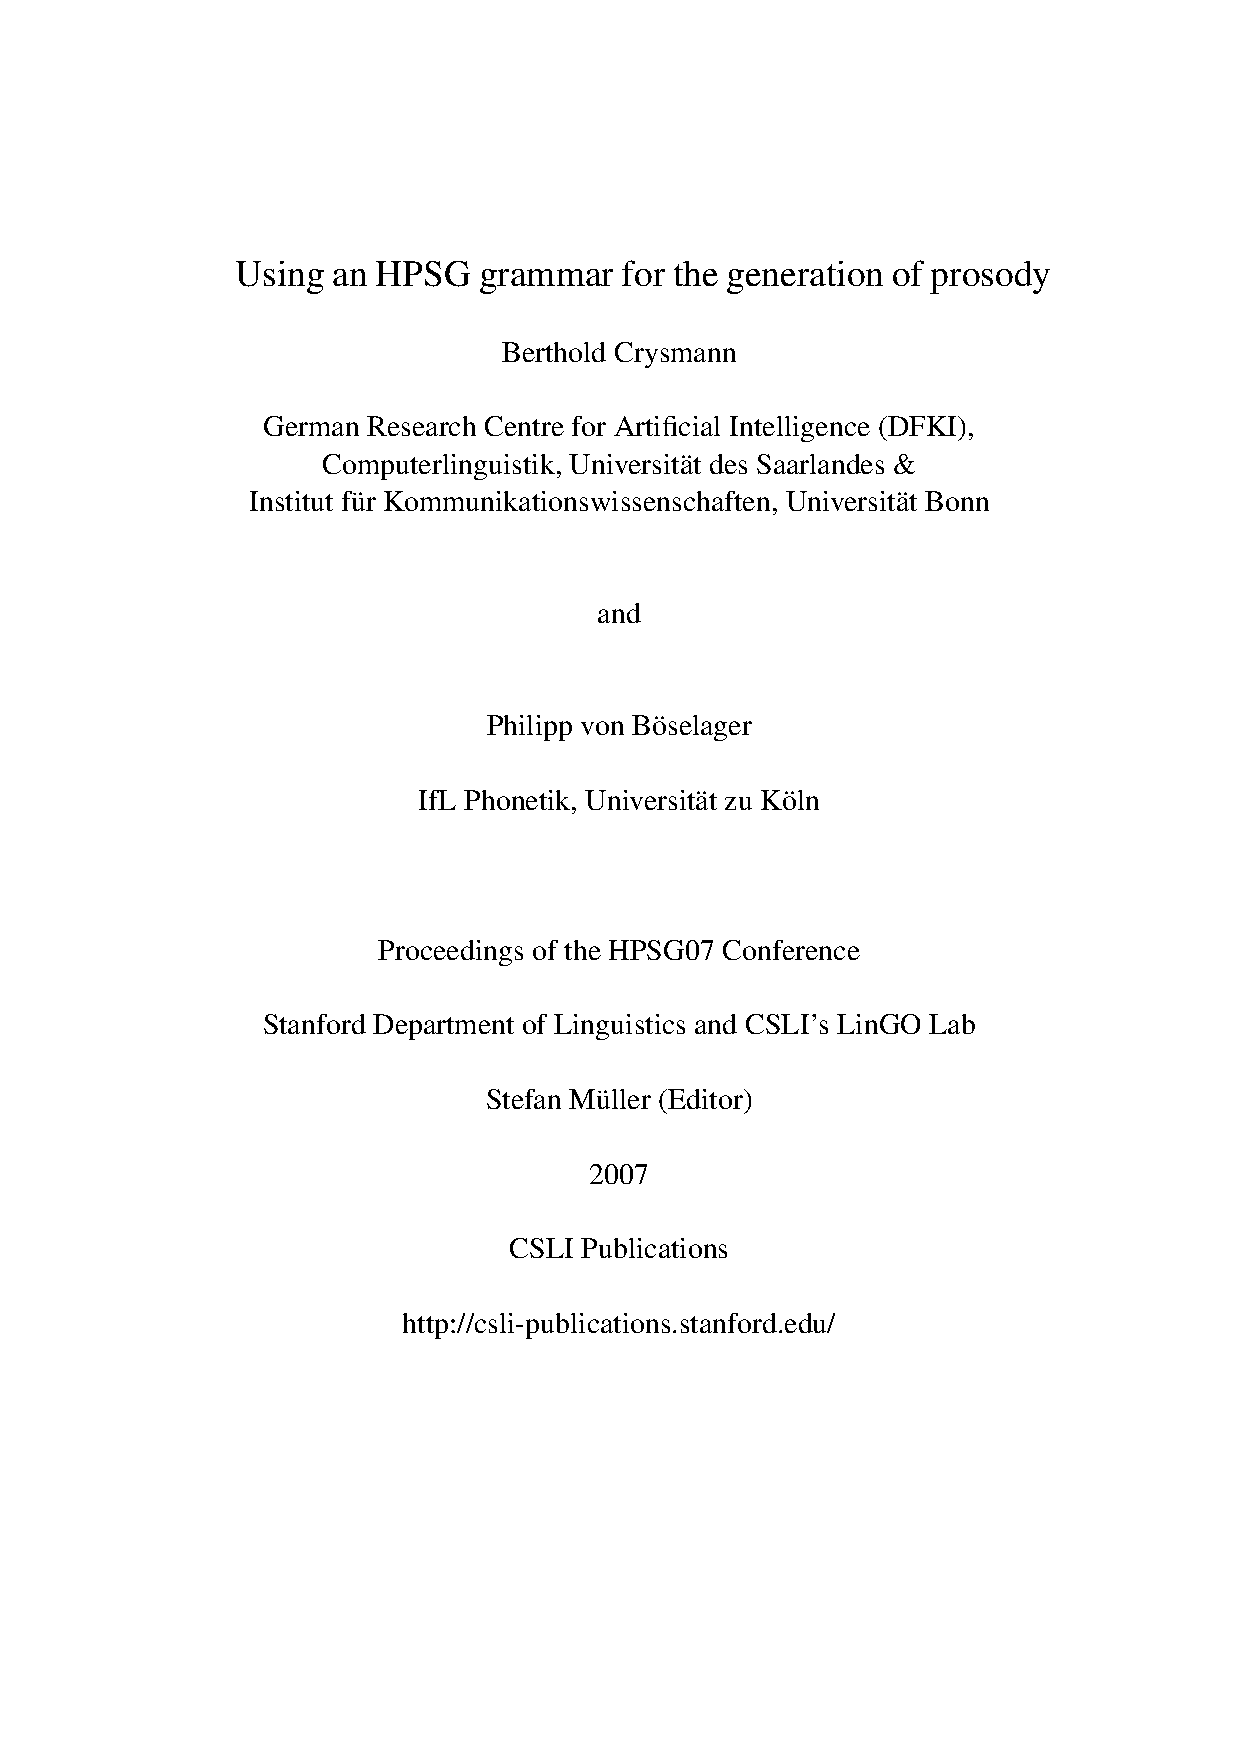
\includepdf[pages=-,pagecommand=\thispagestyle{plain},
            addtotoc={1,section,1,
            {Berthold Crysmann and Philipp von B�selager: Using an HPSG Grammar for the Generation of Prosody},
             crysmann}]{crysmann-boeselager.pdf}


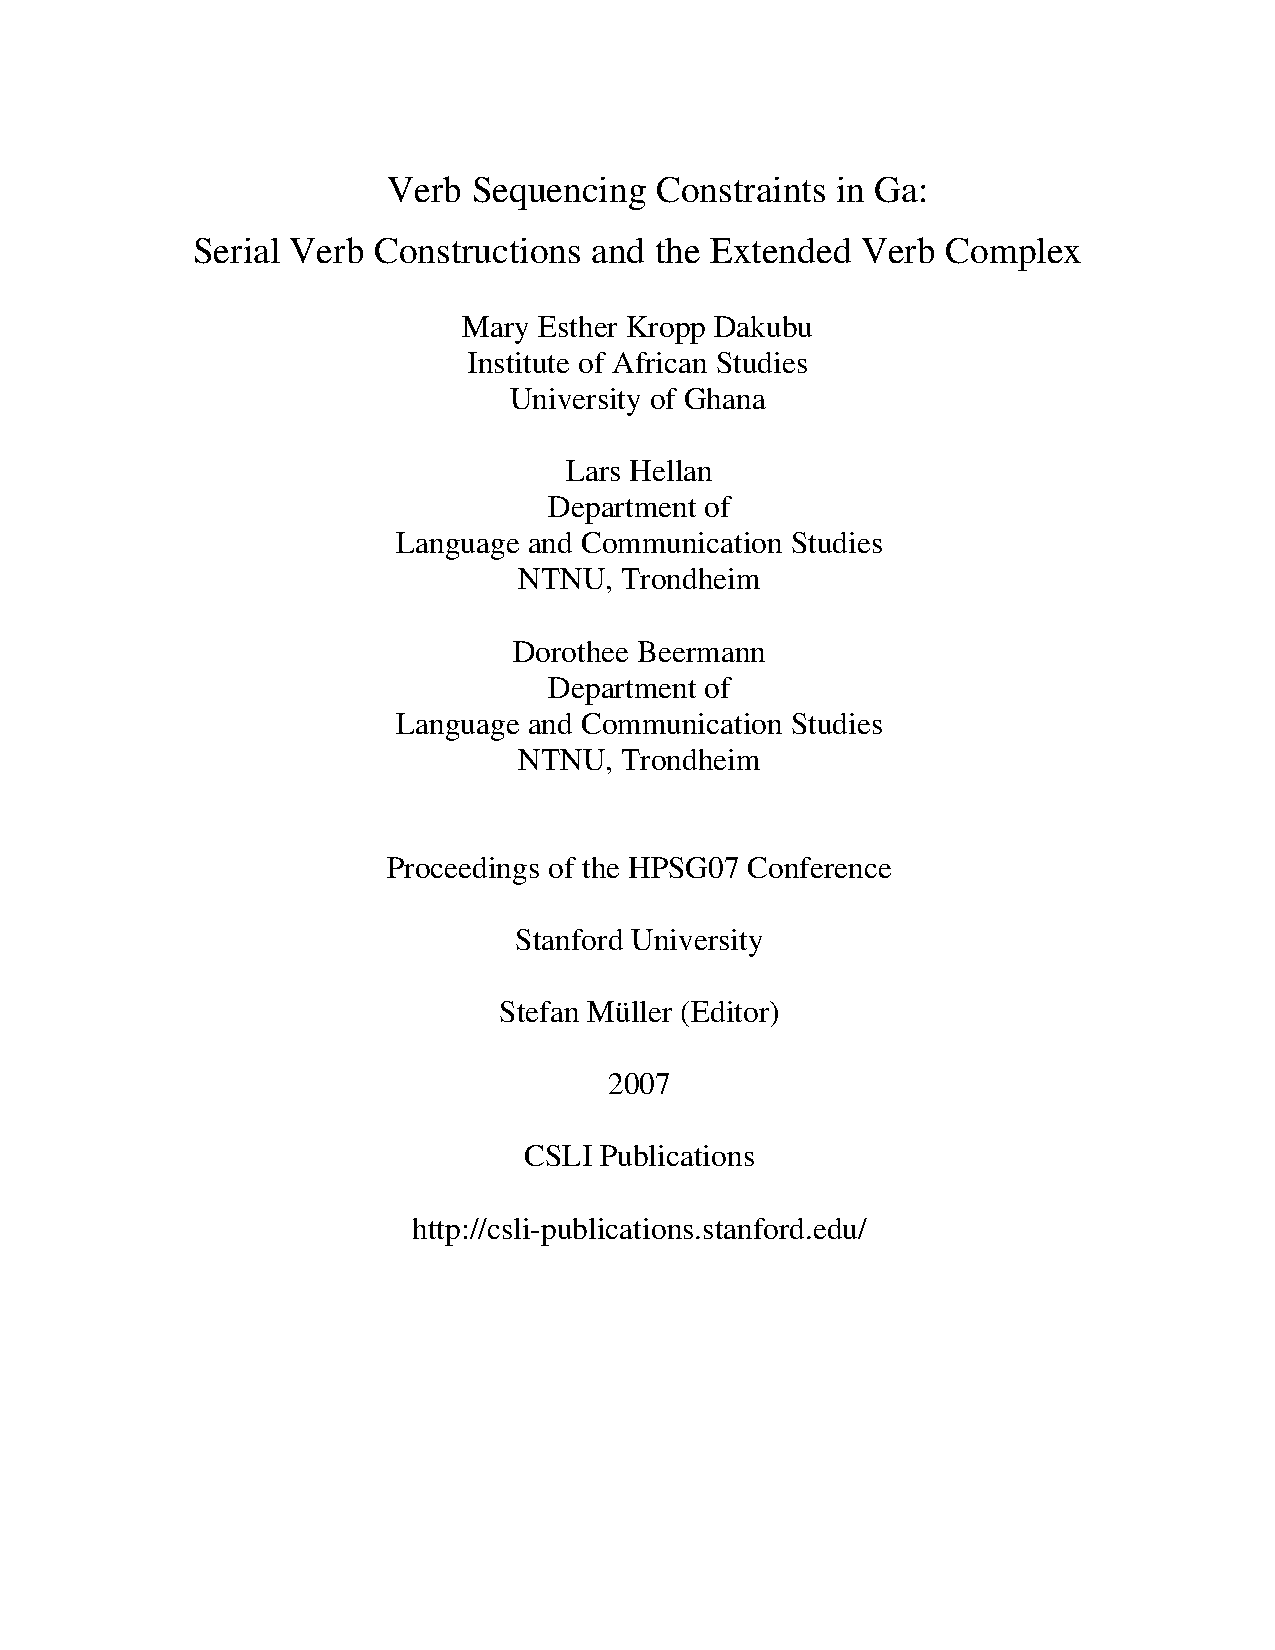
\includepdf[pages=-,pagecommand=\thispagestyle{plain},
            addtotoc={1,section,1,
            {Mary Esther Kropp Dakubu, Lars Hellan and Dorothee Beermann: Verb Sequencing Constraints in Ga:
Serial Verb Constructions and the Extended Verb Complex},
             dhb}]{dakubu-hellan-beermann.pdf}

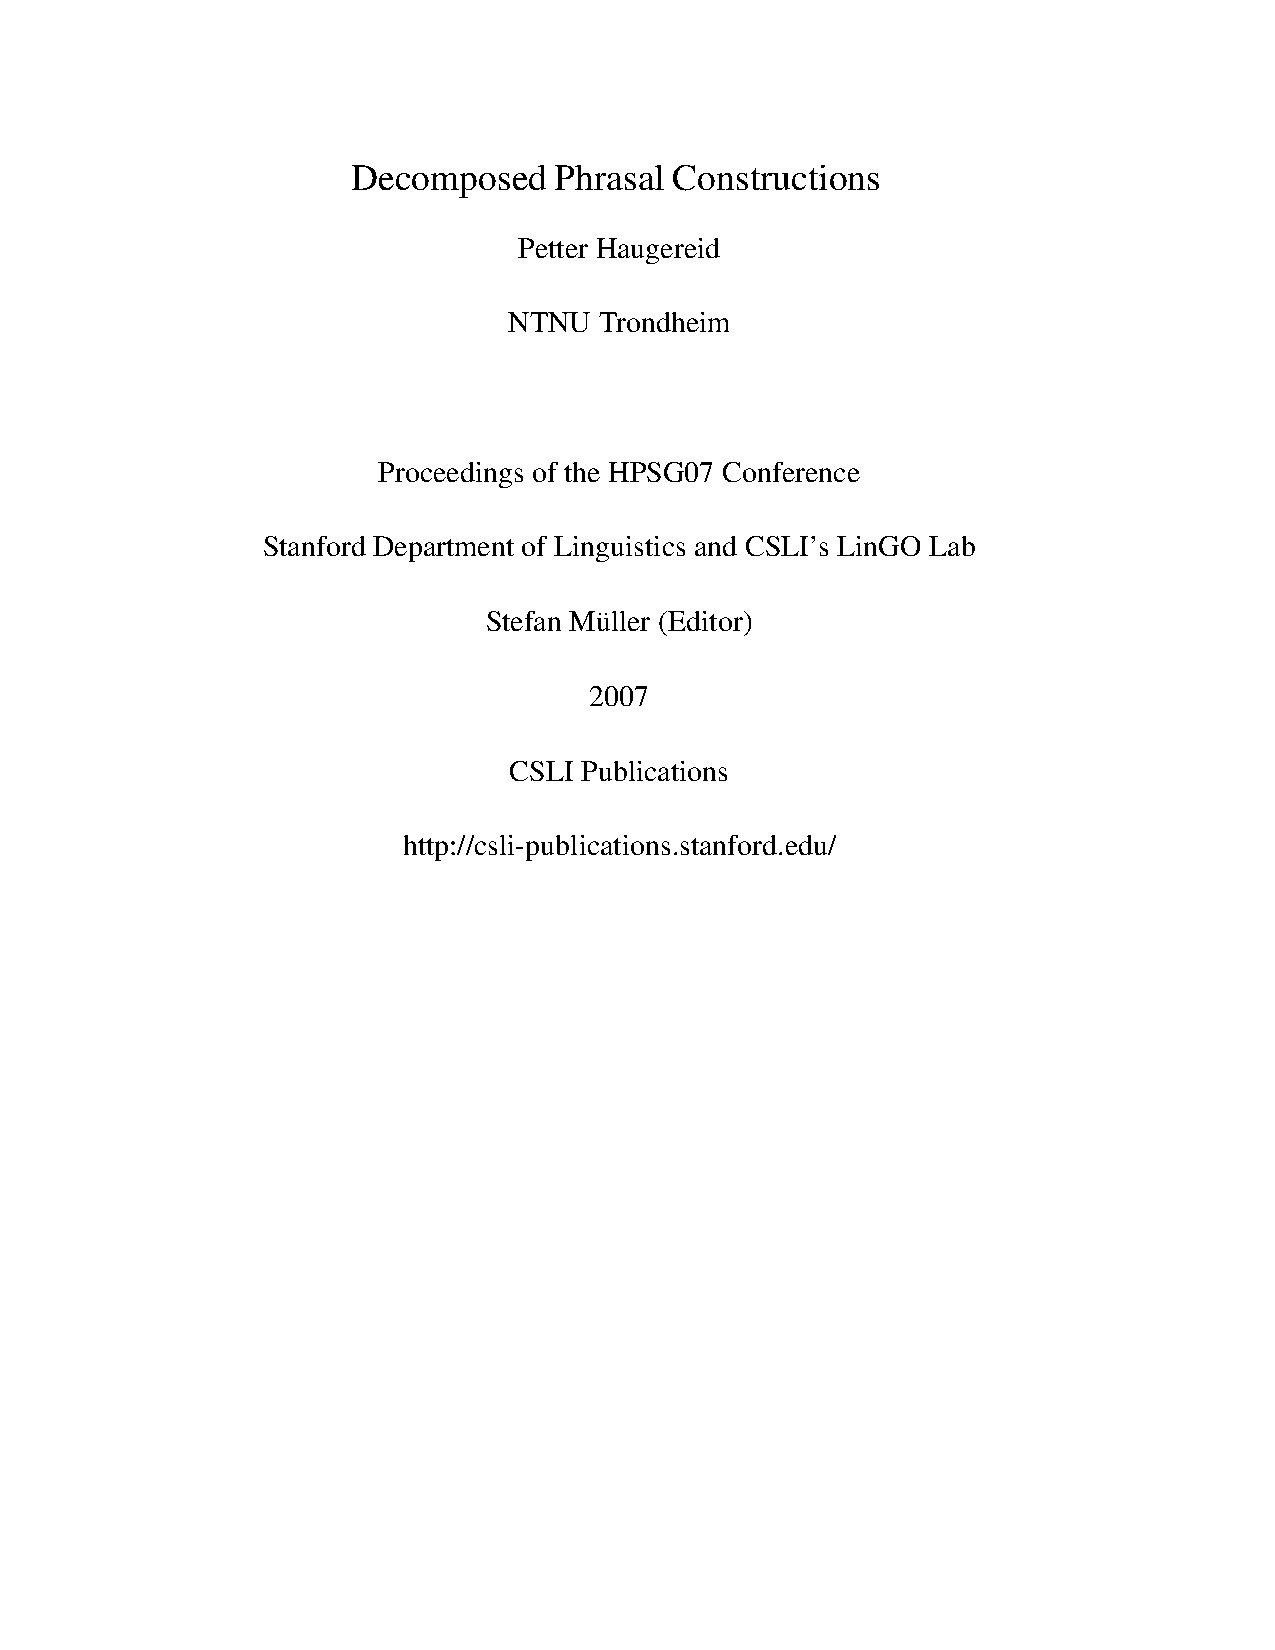
\includepdf[pages=-,pagecommand=\thispagestyle{plain},
            addtotoc={1,section,1,
            {Petter Haugereid: Decomposed Phrasal Constructions},
             haugereid}]{haugereid.pdf}

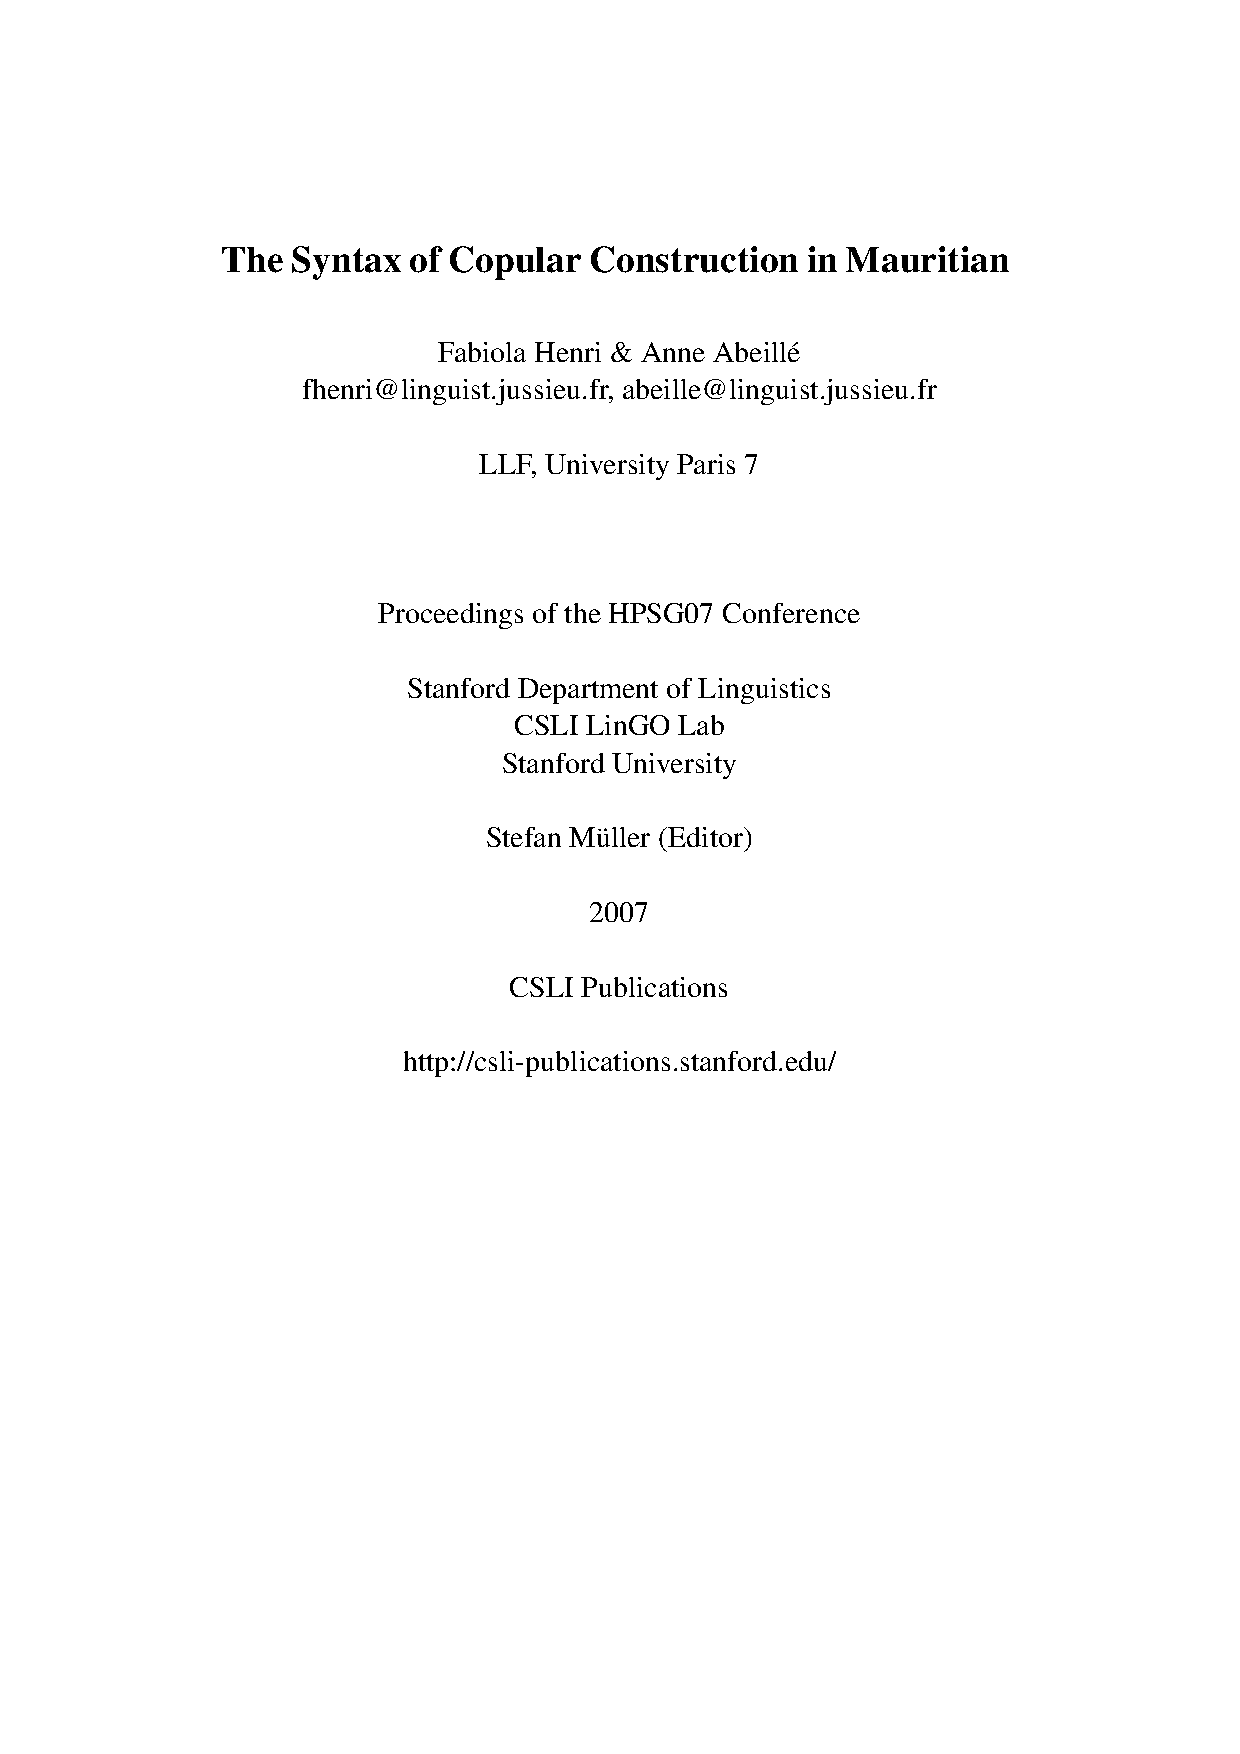
\includepdf[pages=-,pagecommand=\thispagestyle{plain},
            addtotoc={1,section,1,
            {Fabiola Henri and Anne Abeill�: The Syntax of Copular Constructions in Mauritian},
             ha}]{henri-abeille.pdf}

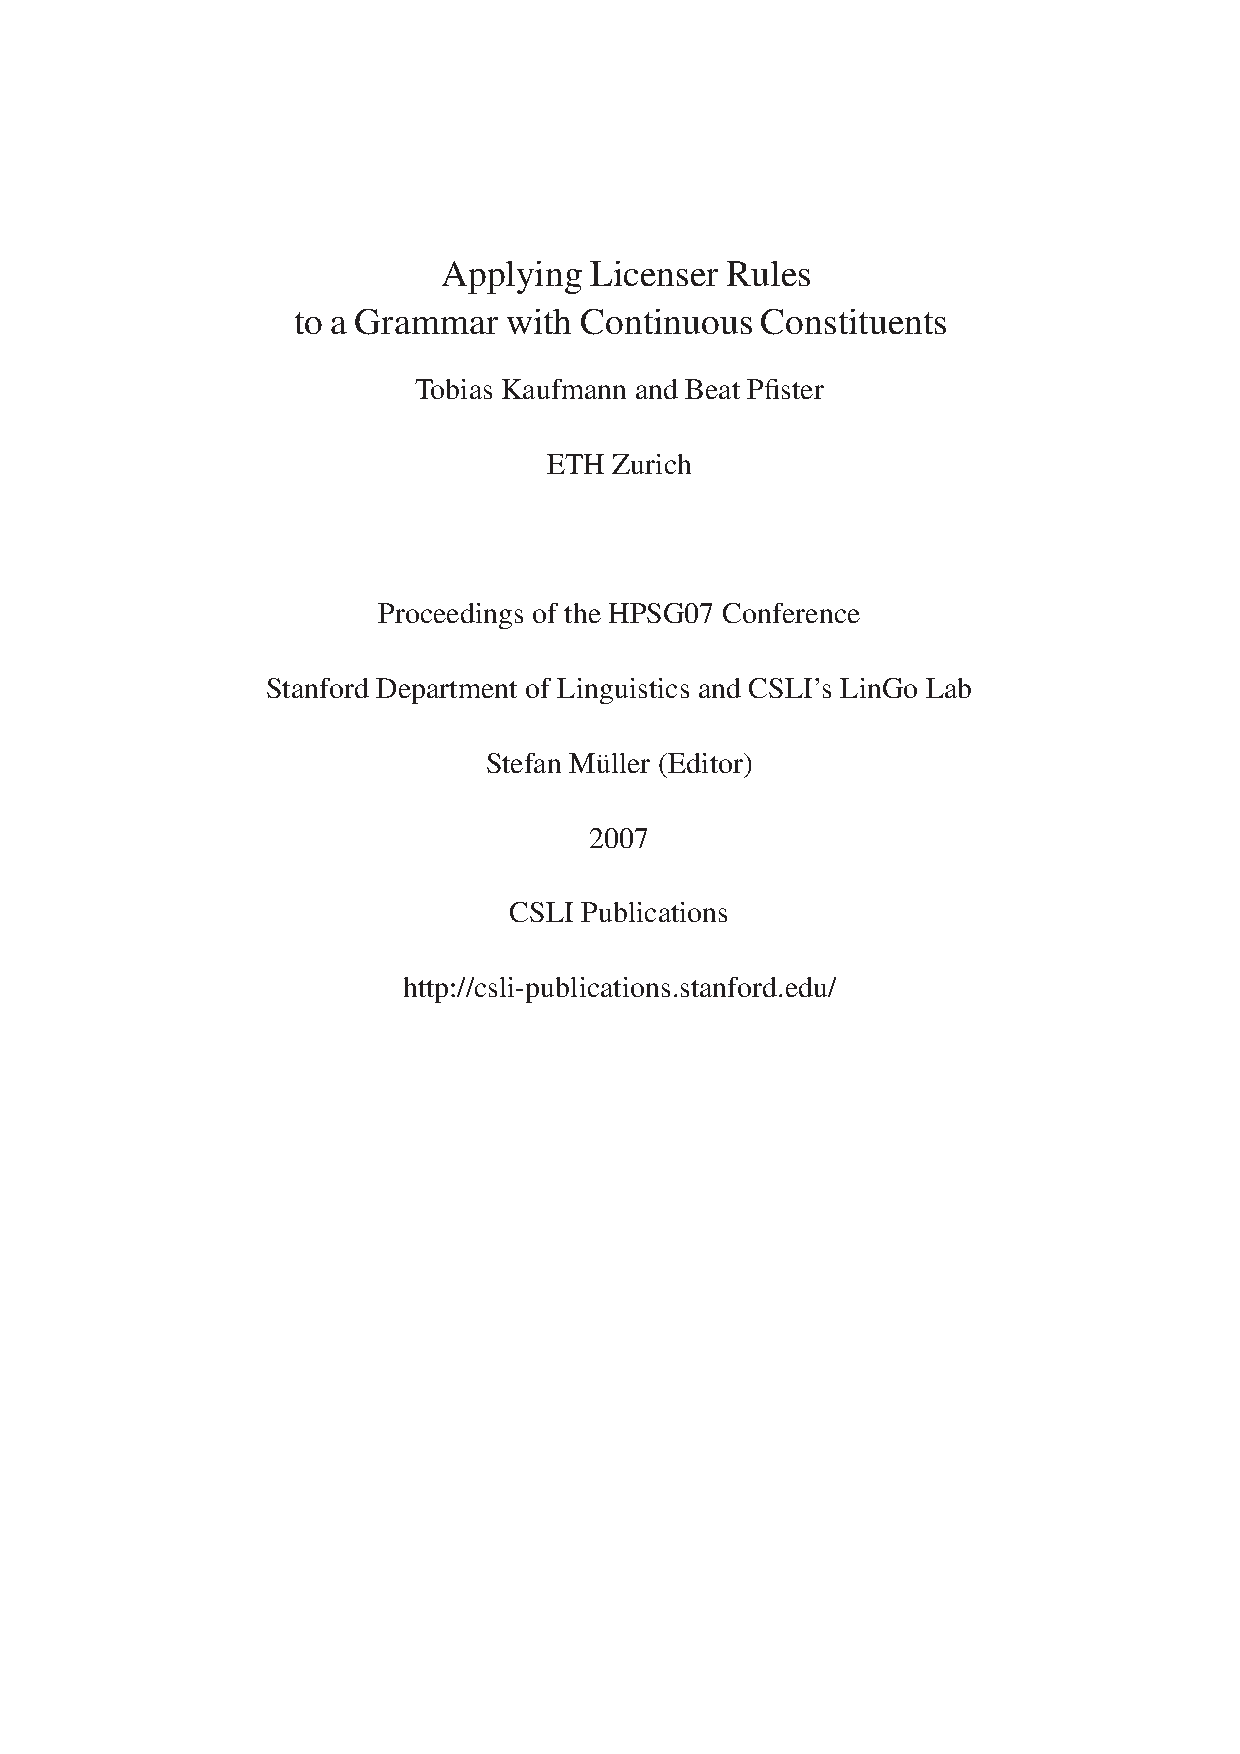
\includepdf[pages=-,pagecommand=\thispagestyle{plain},
            addtotoc={1,section,1,
            {Tobias Kaufmann and Beat Pfister: Applying Licenser Rules to a Grammar with Continuous Constituents},
             kp}]{kaufmann-pfister.pdf}

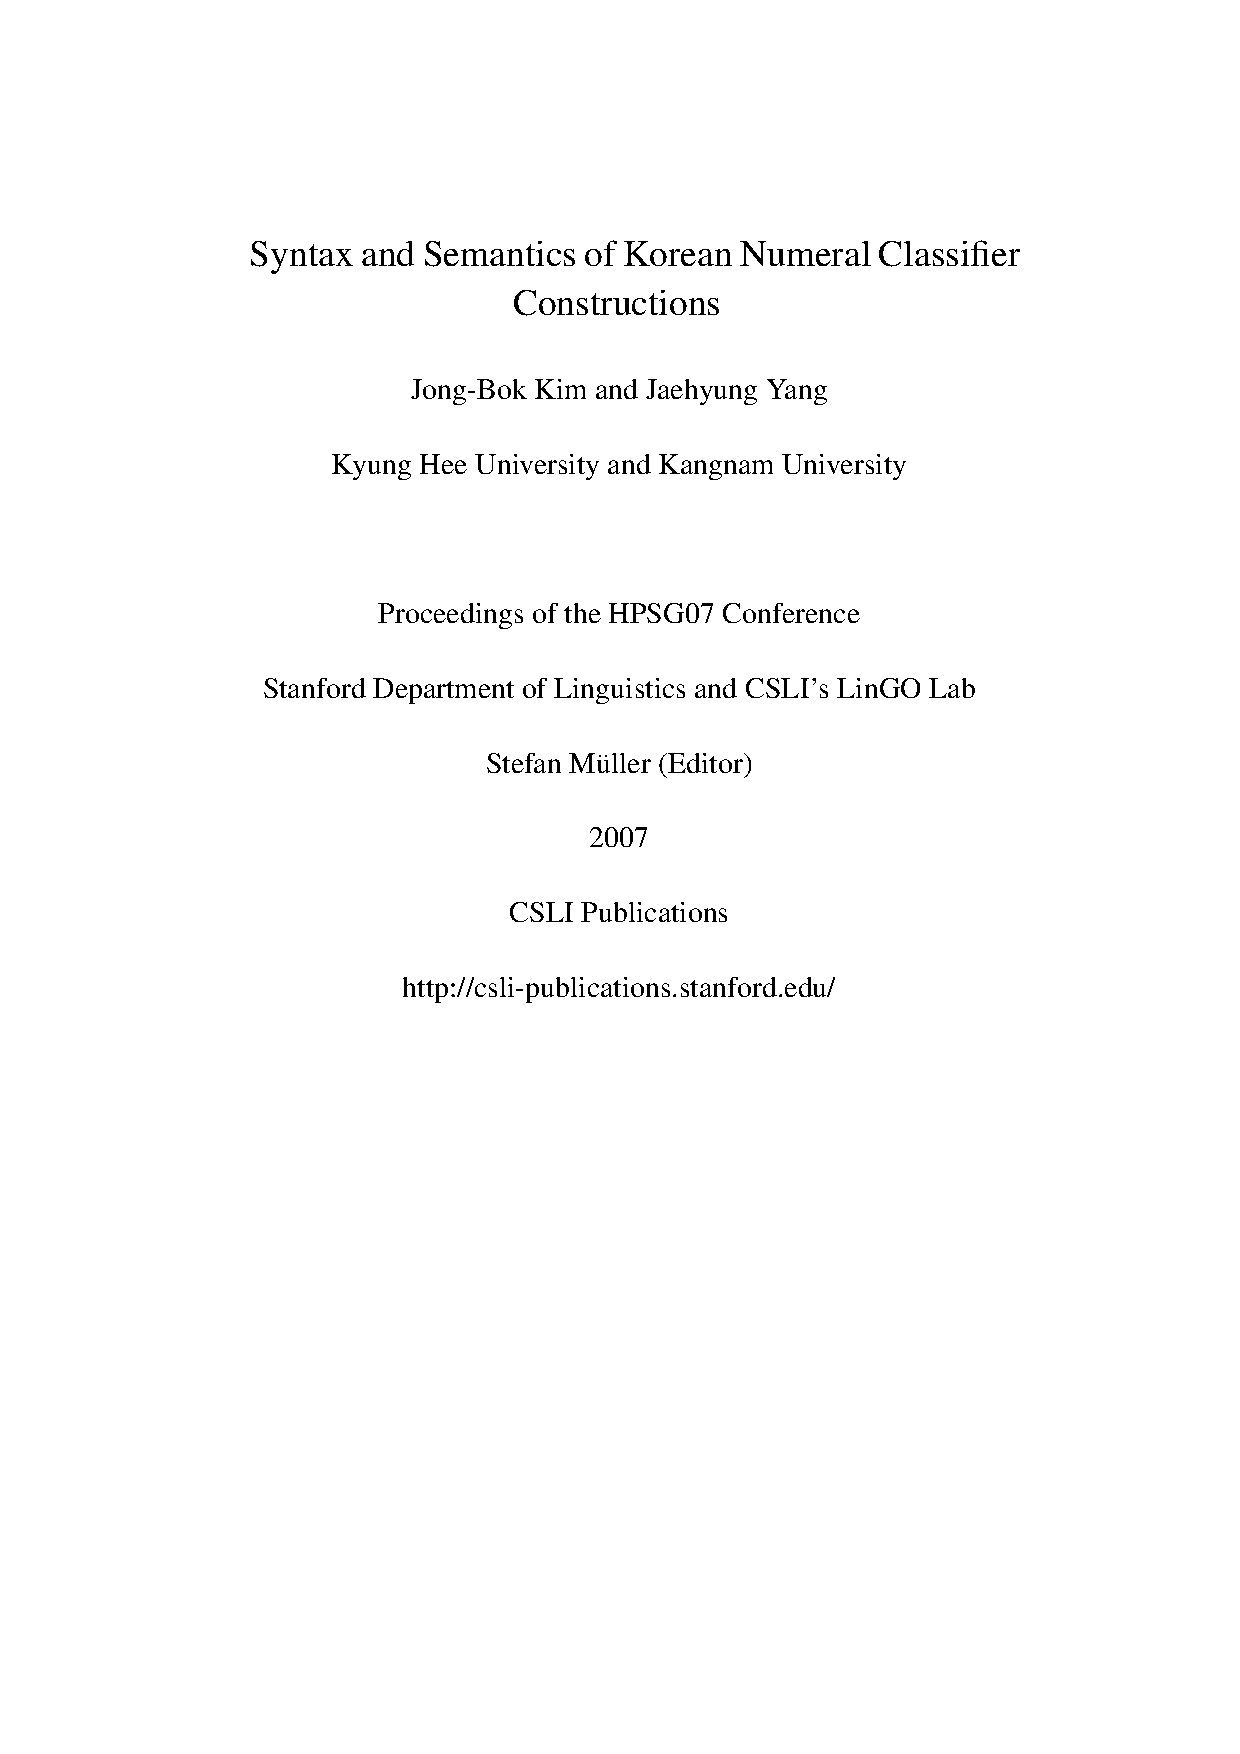
\includepdf[pages=-,pagecommand=\thispagestyle{plain},
            addtotoc={1,section,1,
            {Jong-Bok Kim and Jaehyung Yang: Syntax and Semantics of Korean Numeral Classifier Constructions},
             ky}]{kim-yang.pdf}



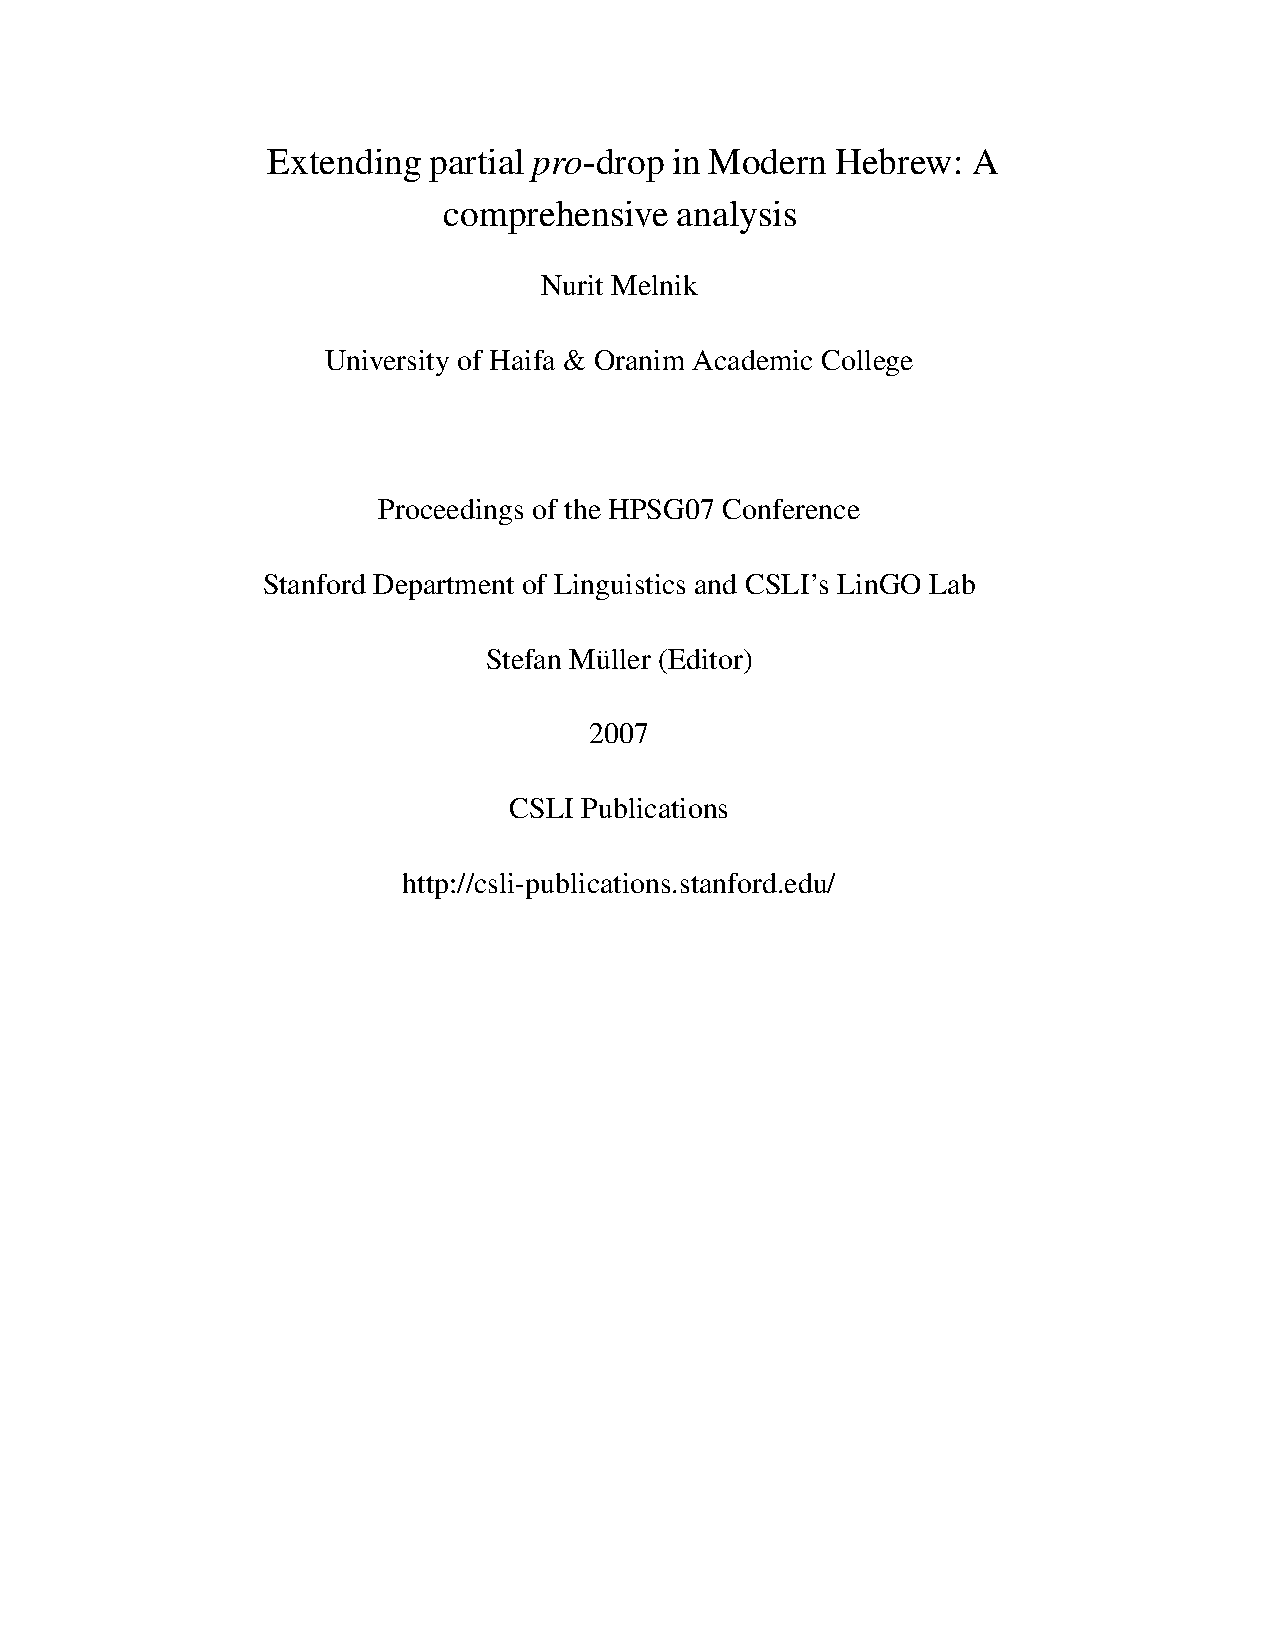
\includepdf[pages=-,pagecommand=\thispagestyle{plain},
            addtotoc={1,section,1,
            {Nurit Melnik: Extending Partial Pro-drop in Modern Hebrew: A Comprehensive Analysis},
             melnik}]{melnik.pdf}

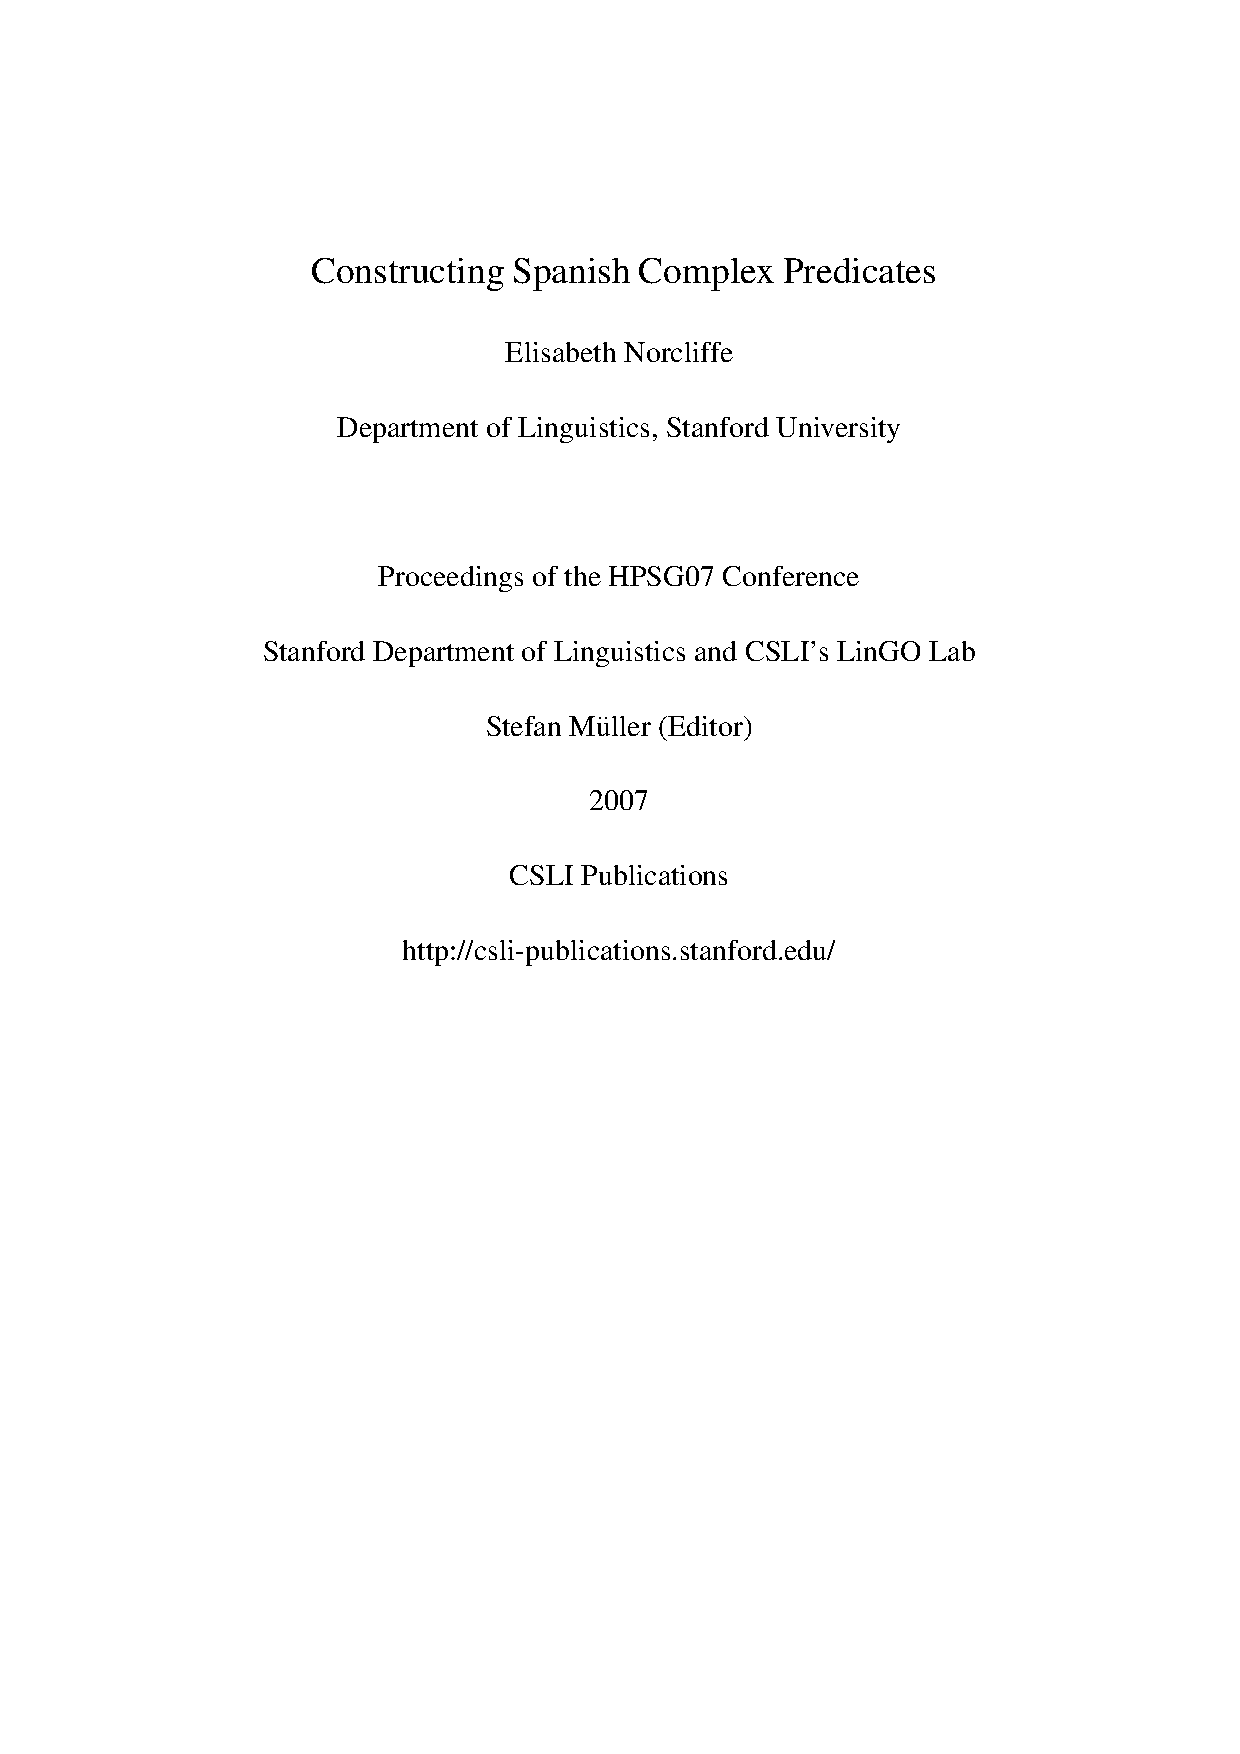
\includepdf[pages=-,pagecommand=\thispagestyle{plain},
            addtotoc={1,section,1,
            {Elisabeth Norcliffe: Constructing Spanish Complex Predicates},
             norcliffe}]{norcliffe.pdf}

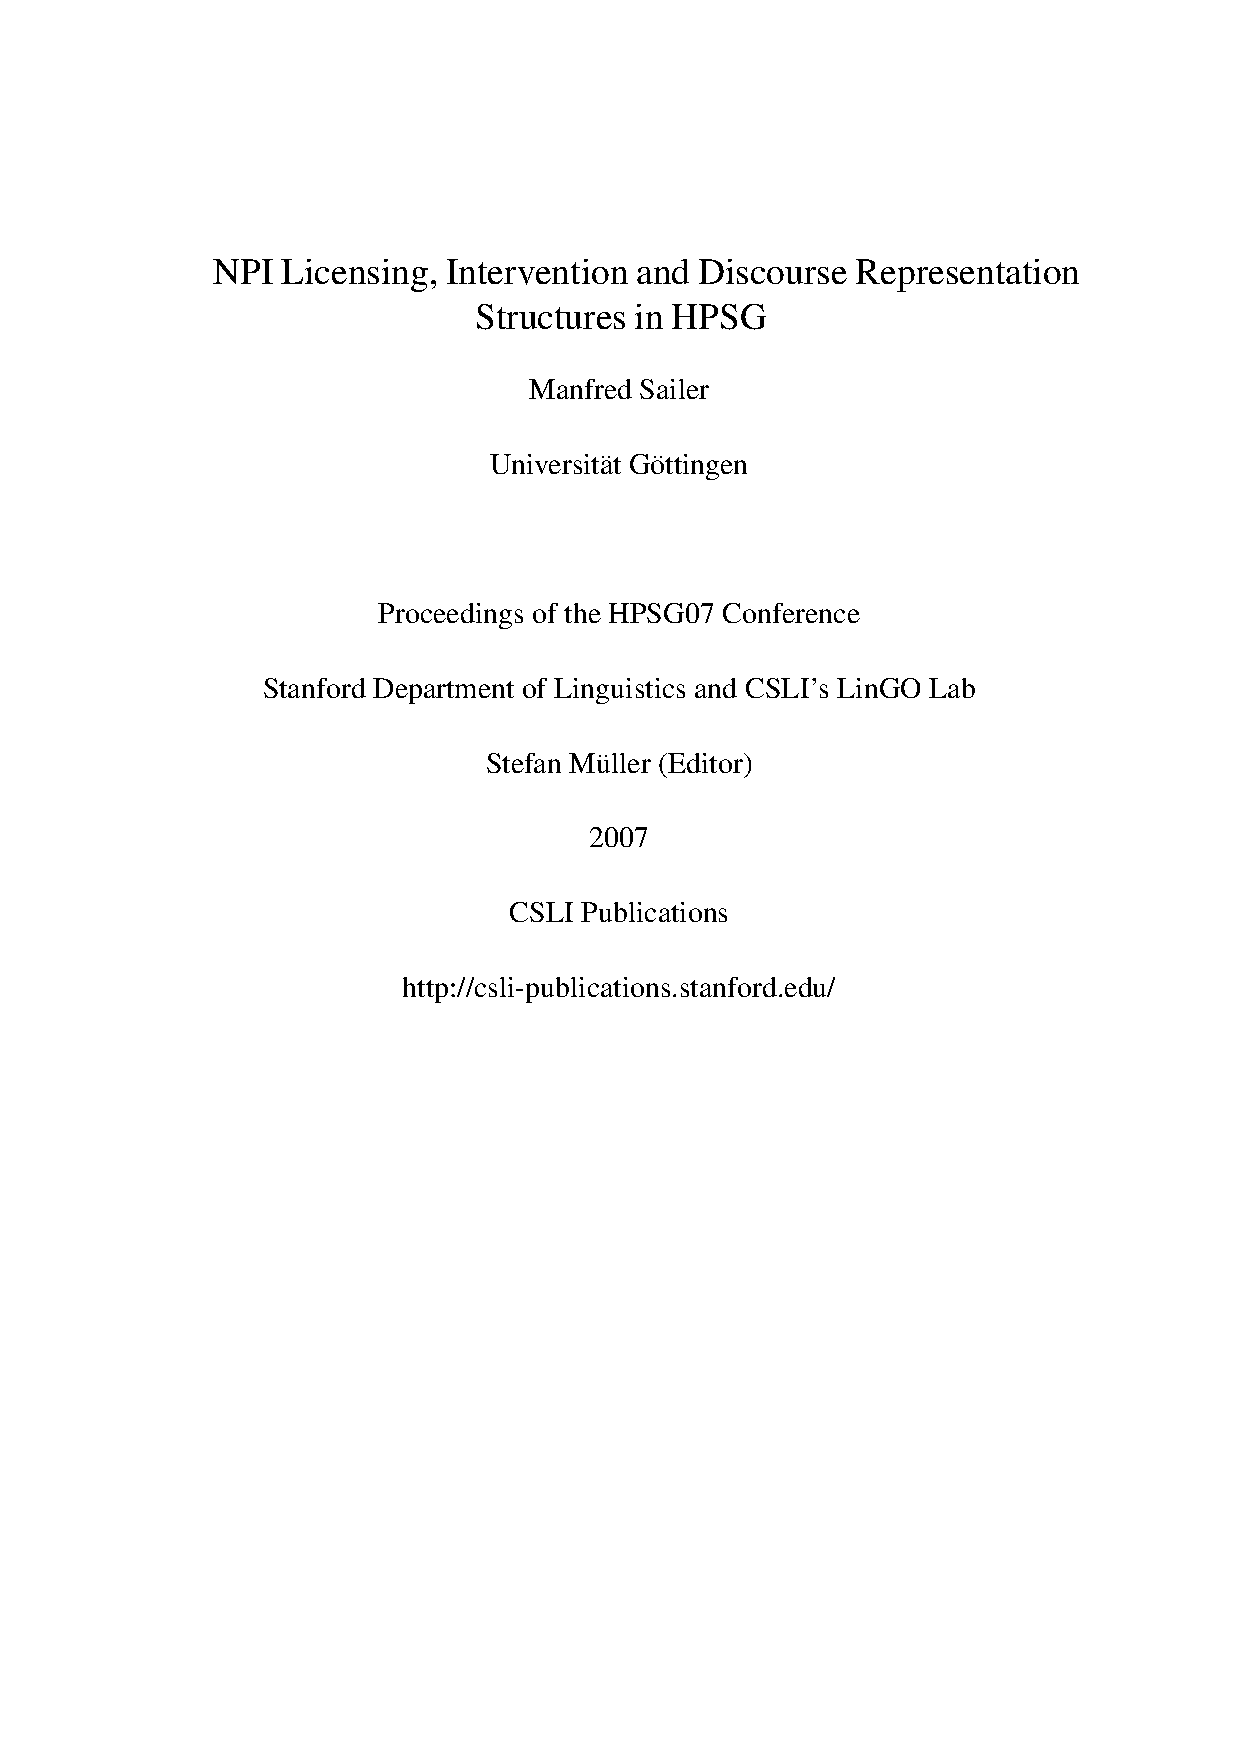
\includepdf[pages=-,pagecommand=\thispagestyle{plain},
            addtotoc={1,section,1,
            {Manfred Sailer: NPI Licensing, Intervention and Discourse Representation Structures in HPSG},
             sailer}]{sailer.pdf}

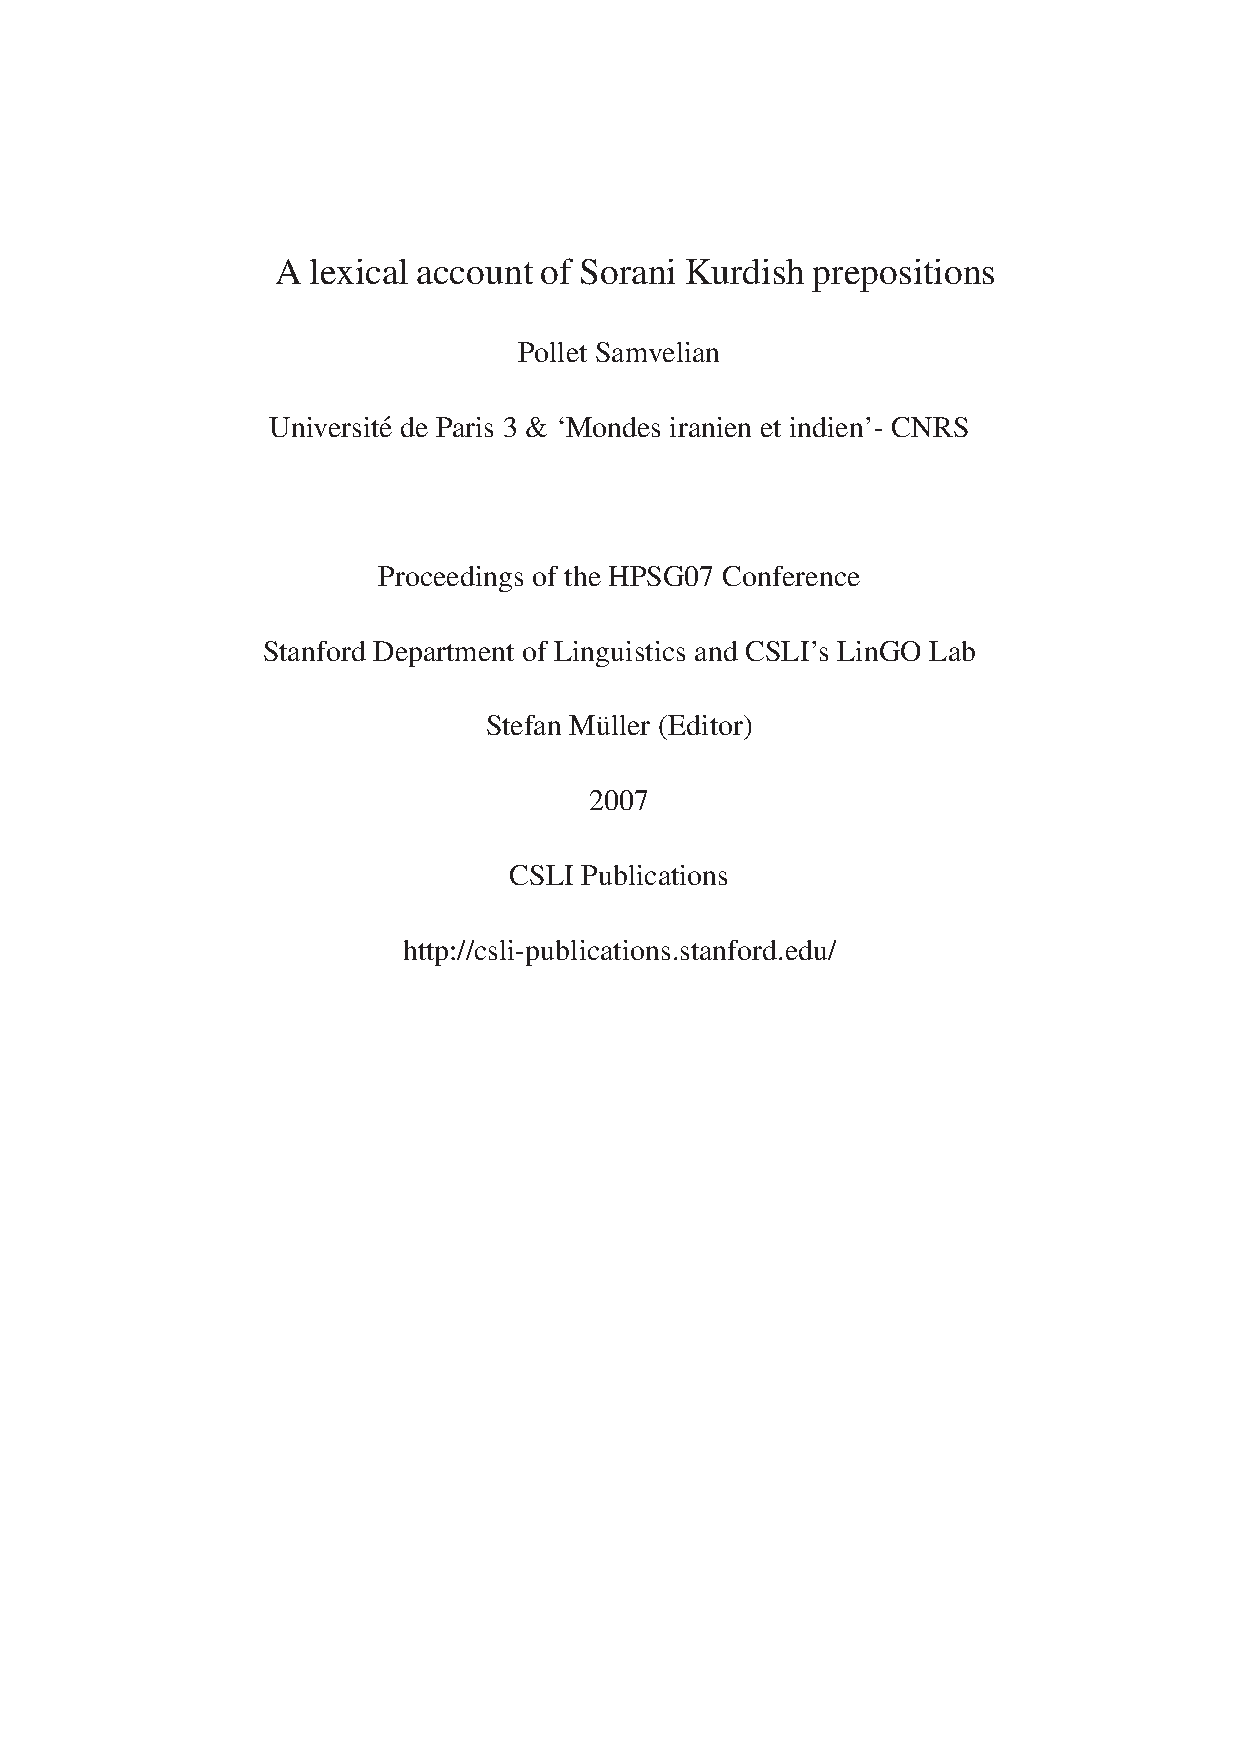
\includepdf[pages=-,pagecommand=\thispagestyle{plain},
            addtotoc={1,section,1,
            {Pollet Samvelian: A Lexical Account of Sorani Kurdish Prepositions},
             samvelian}]{samvelian.pdf}

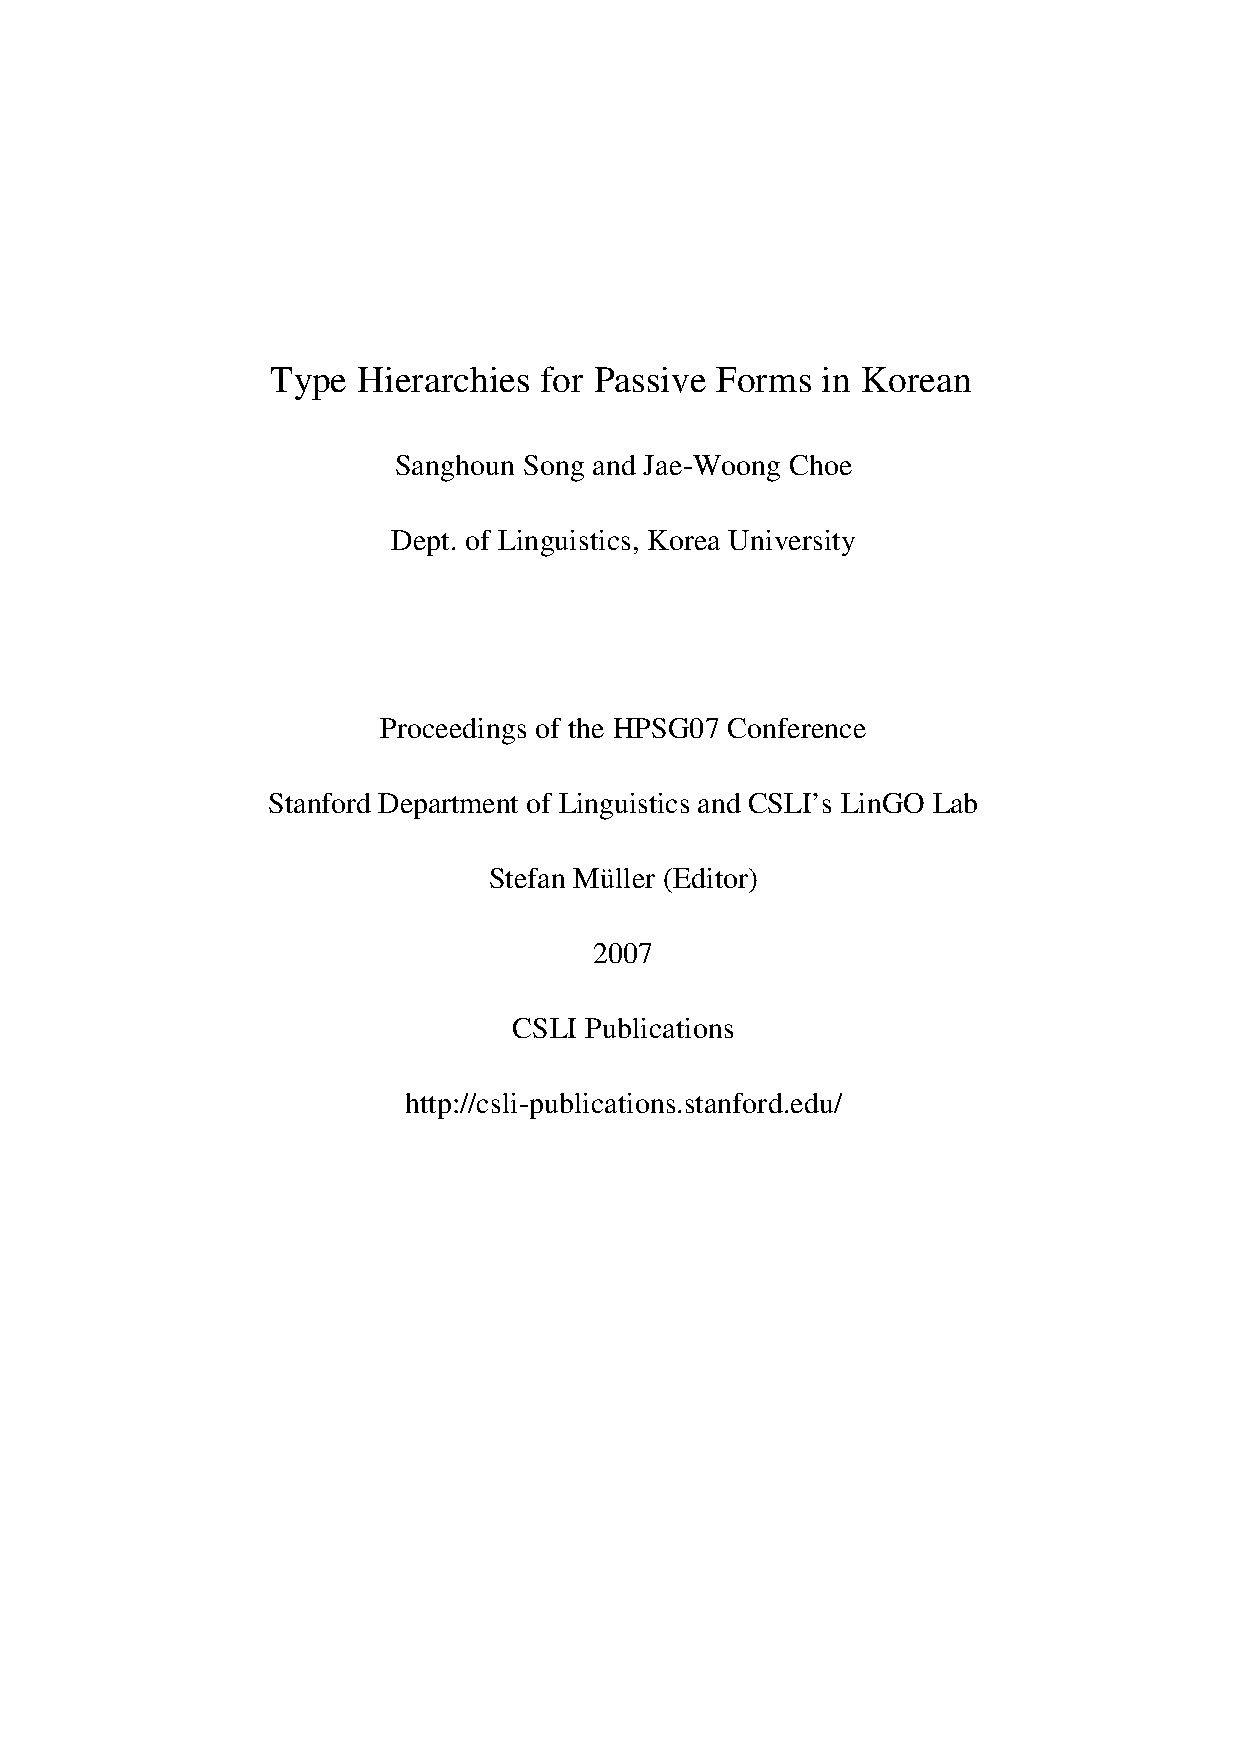
\includepdf[pages=-,pagecommand=\thispagestyle{plain},
            addtotoc={1,section,1,
            {Sanghoun Song and Jae-Woong Choe: Type Hierarchies for Passive Forms in Korean},
             song-choe}]{song-choe.pdf}


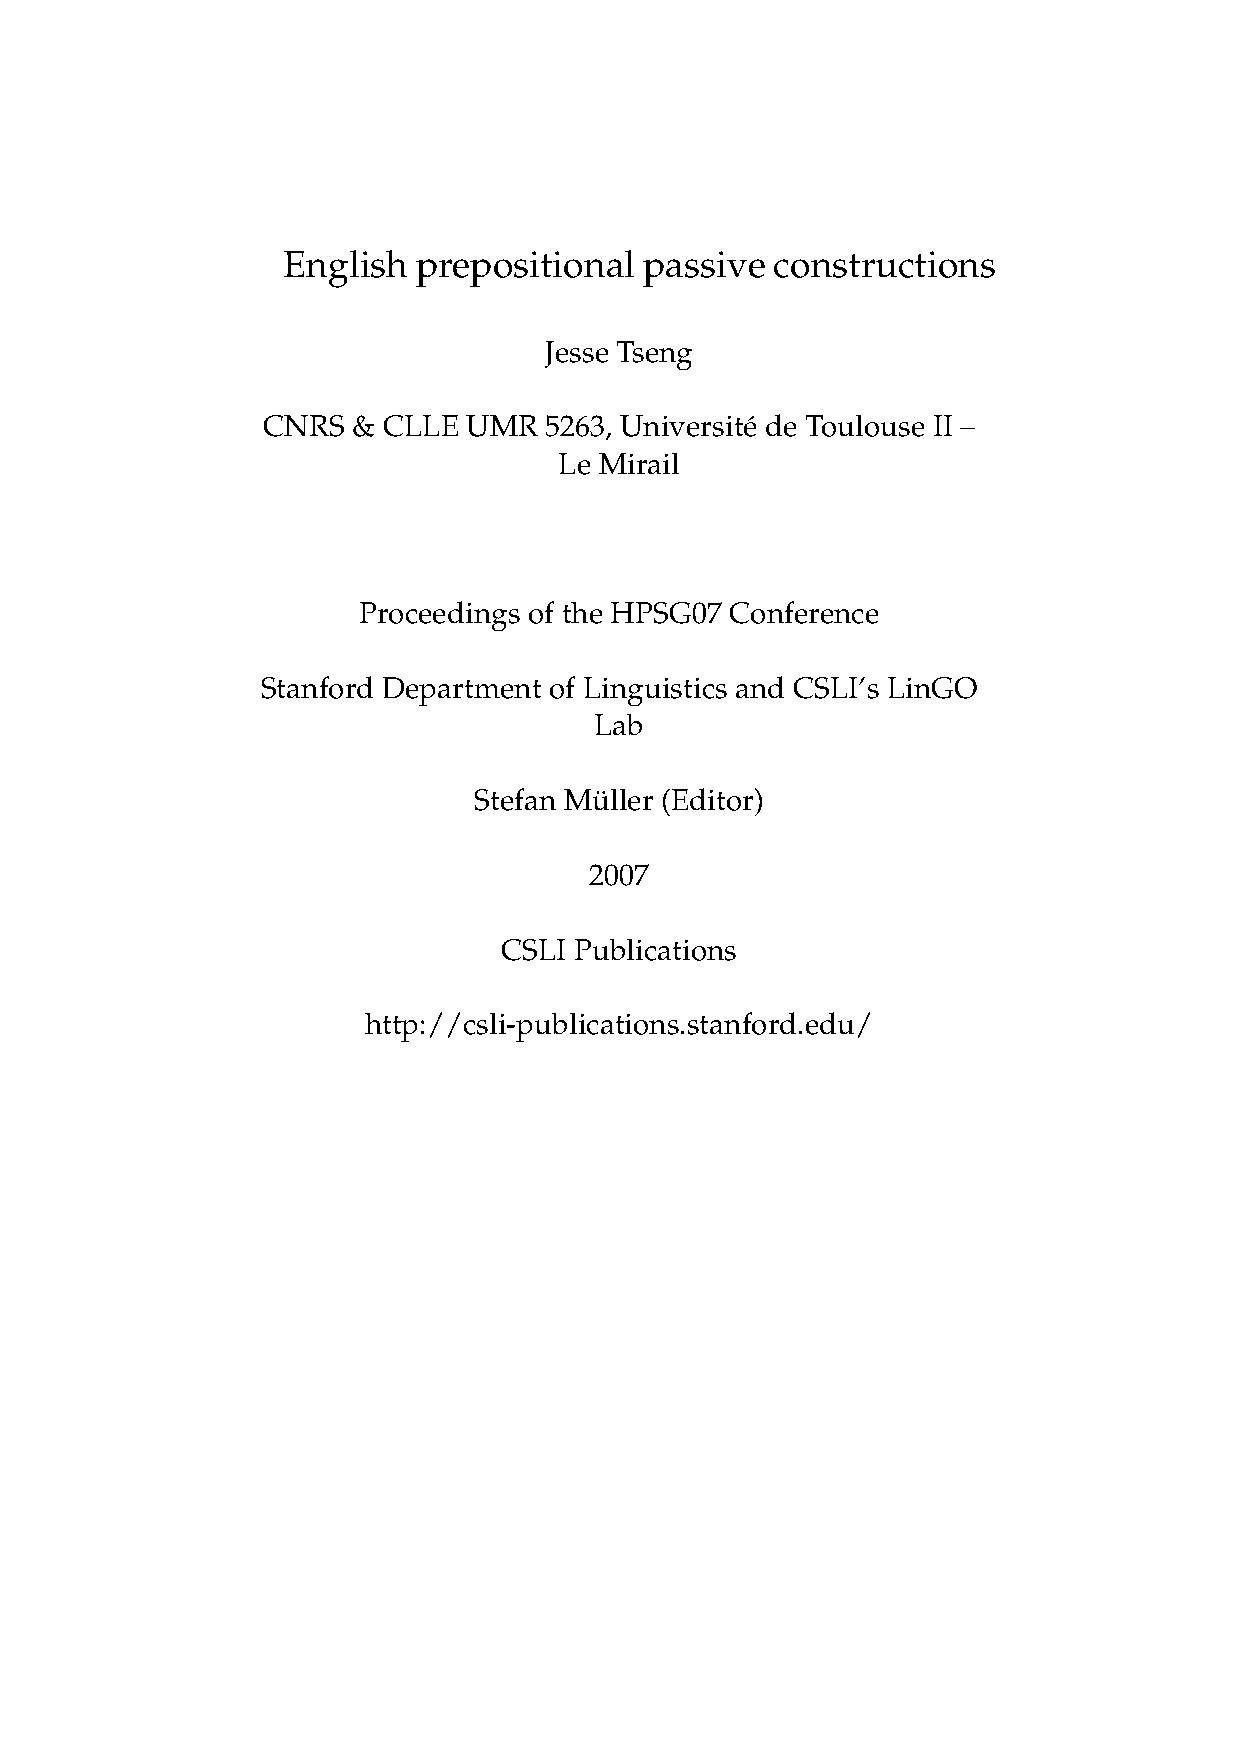
\includepdf[pages=-,pagecommand=\thispagestyle{plain},
            addtotoc={1,section,1,
            {Jesse Tseng: English Prepositional Passive Constructions},
             tseng}]{tseng.pdf}

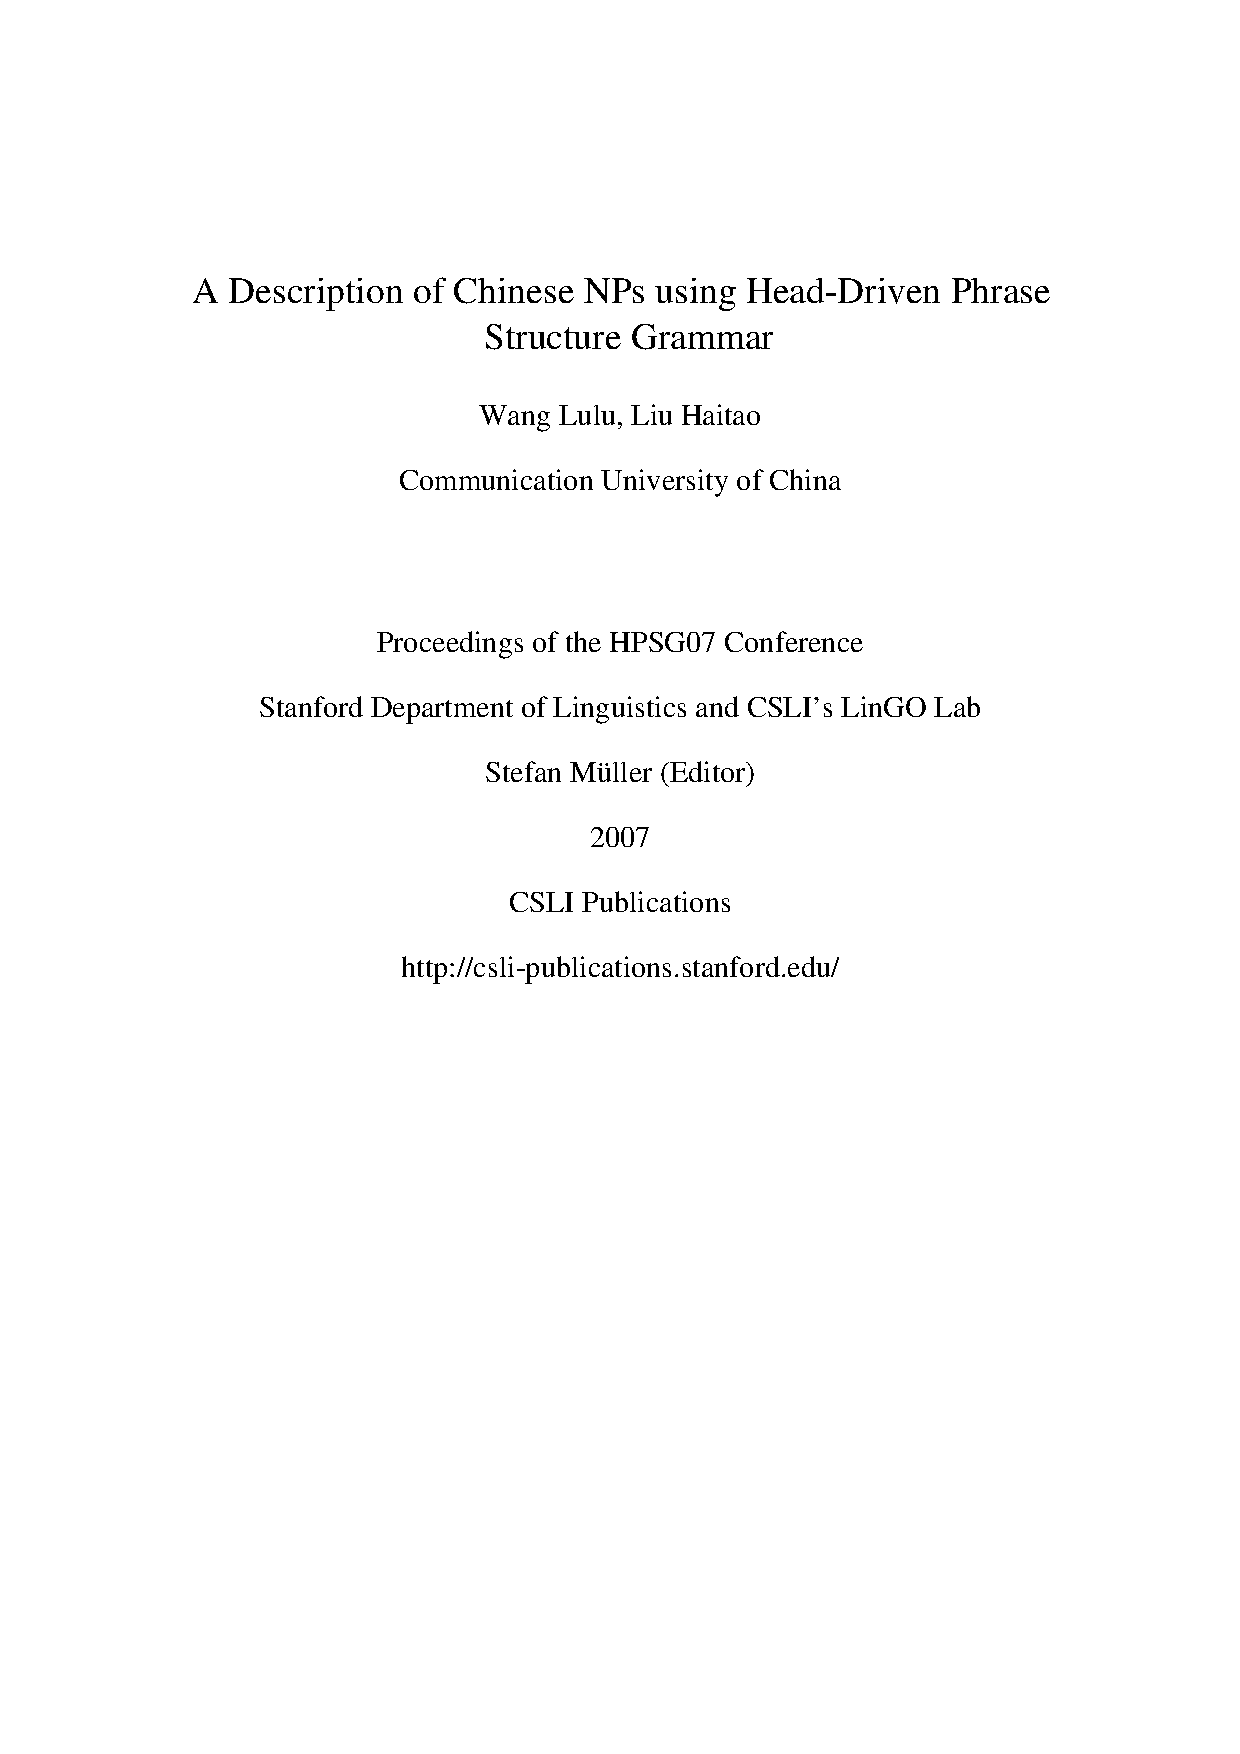
\includepdf[pages=-,pagecommand=\thispagestyle{plain},
            addtotoc={1,section,1,
            {Wang Lulu and Liu Haitao: A Description of Chinese NPs using
Head-Driven Phrase Structure Grammar},
             wang-liu}]{wang-liu.pdf}

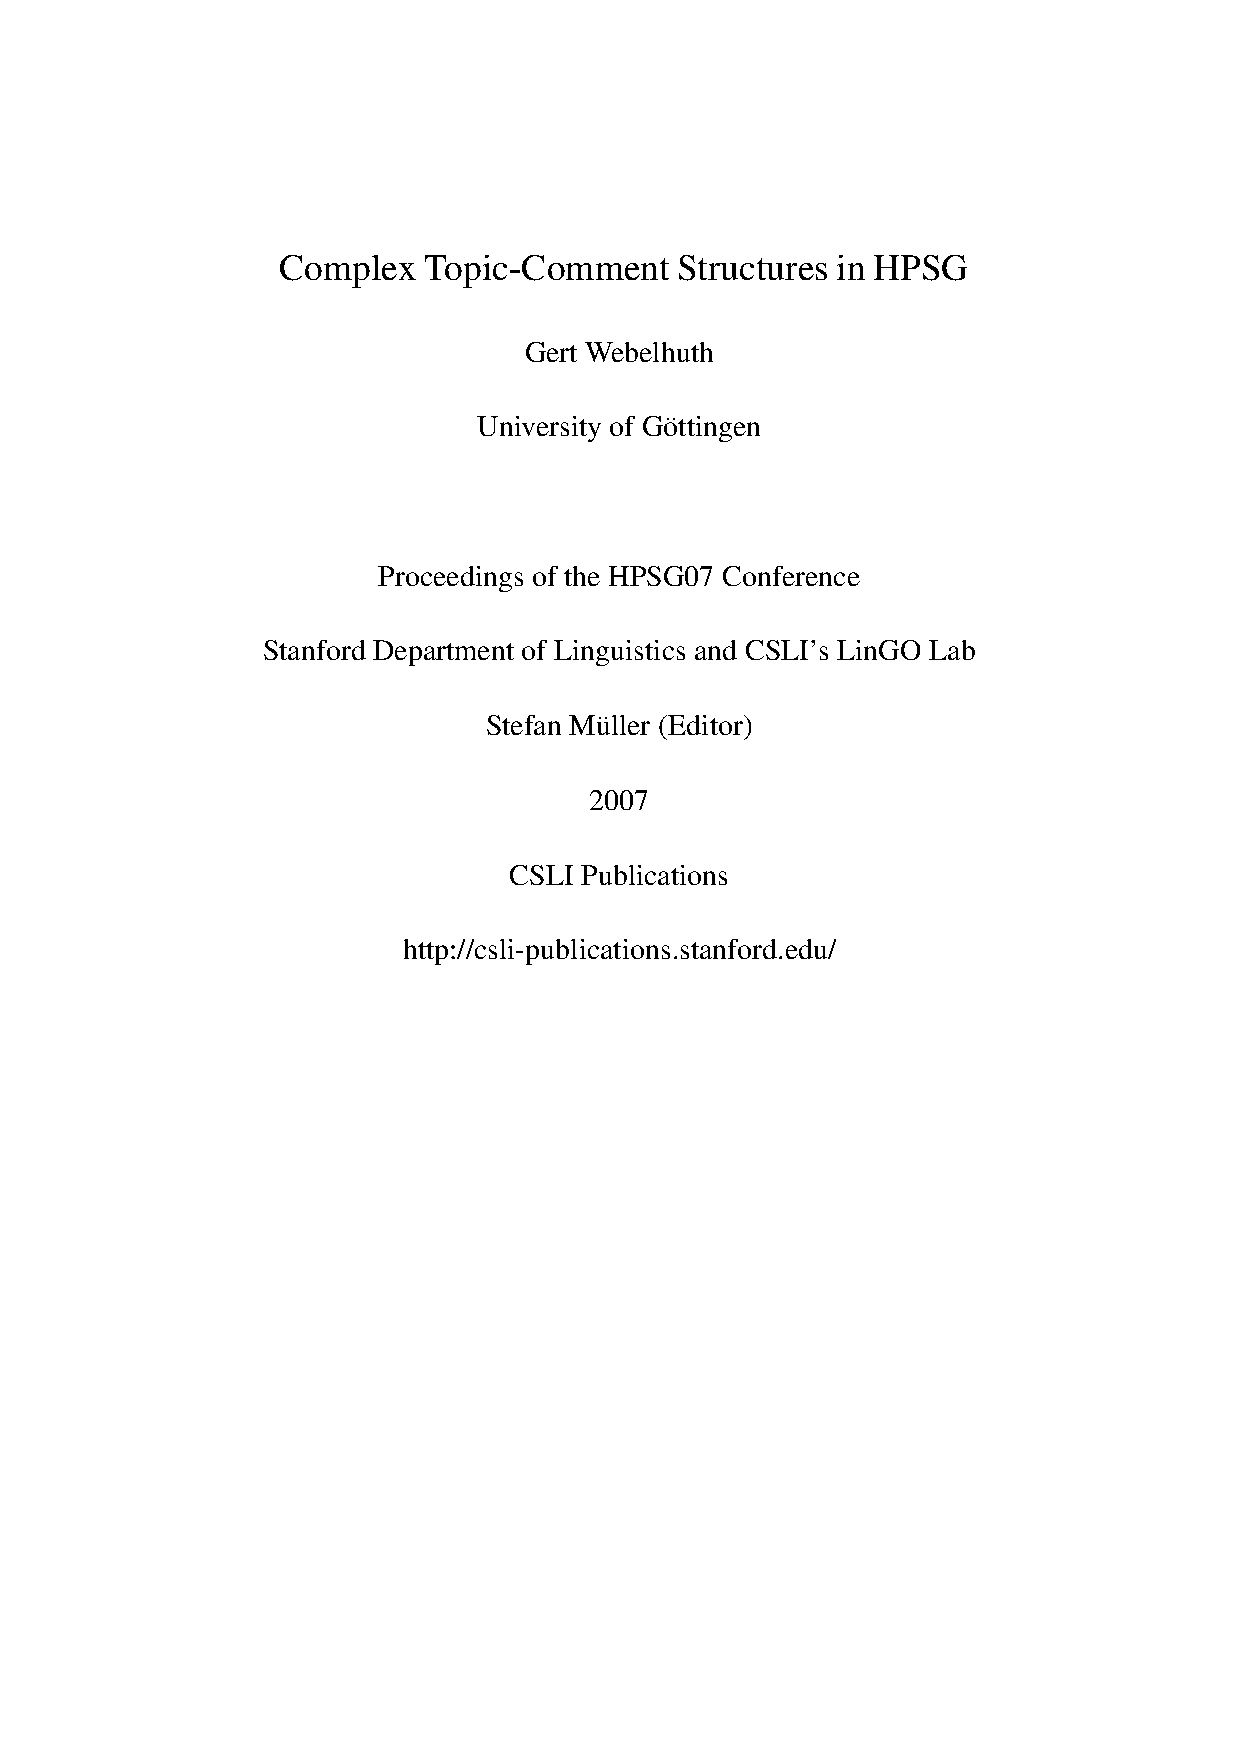
\includepdf[pages=-,pagecommand=\thispagestyle{plain},
            addtotoc={1,section,1,
            {Gert Webelhuth: Complex Topic-Comment Structures in HPSG},
             webelhuth}]{webelhuth.pdf}

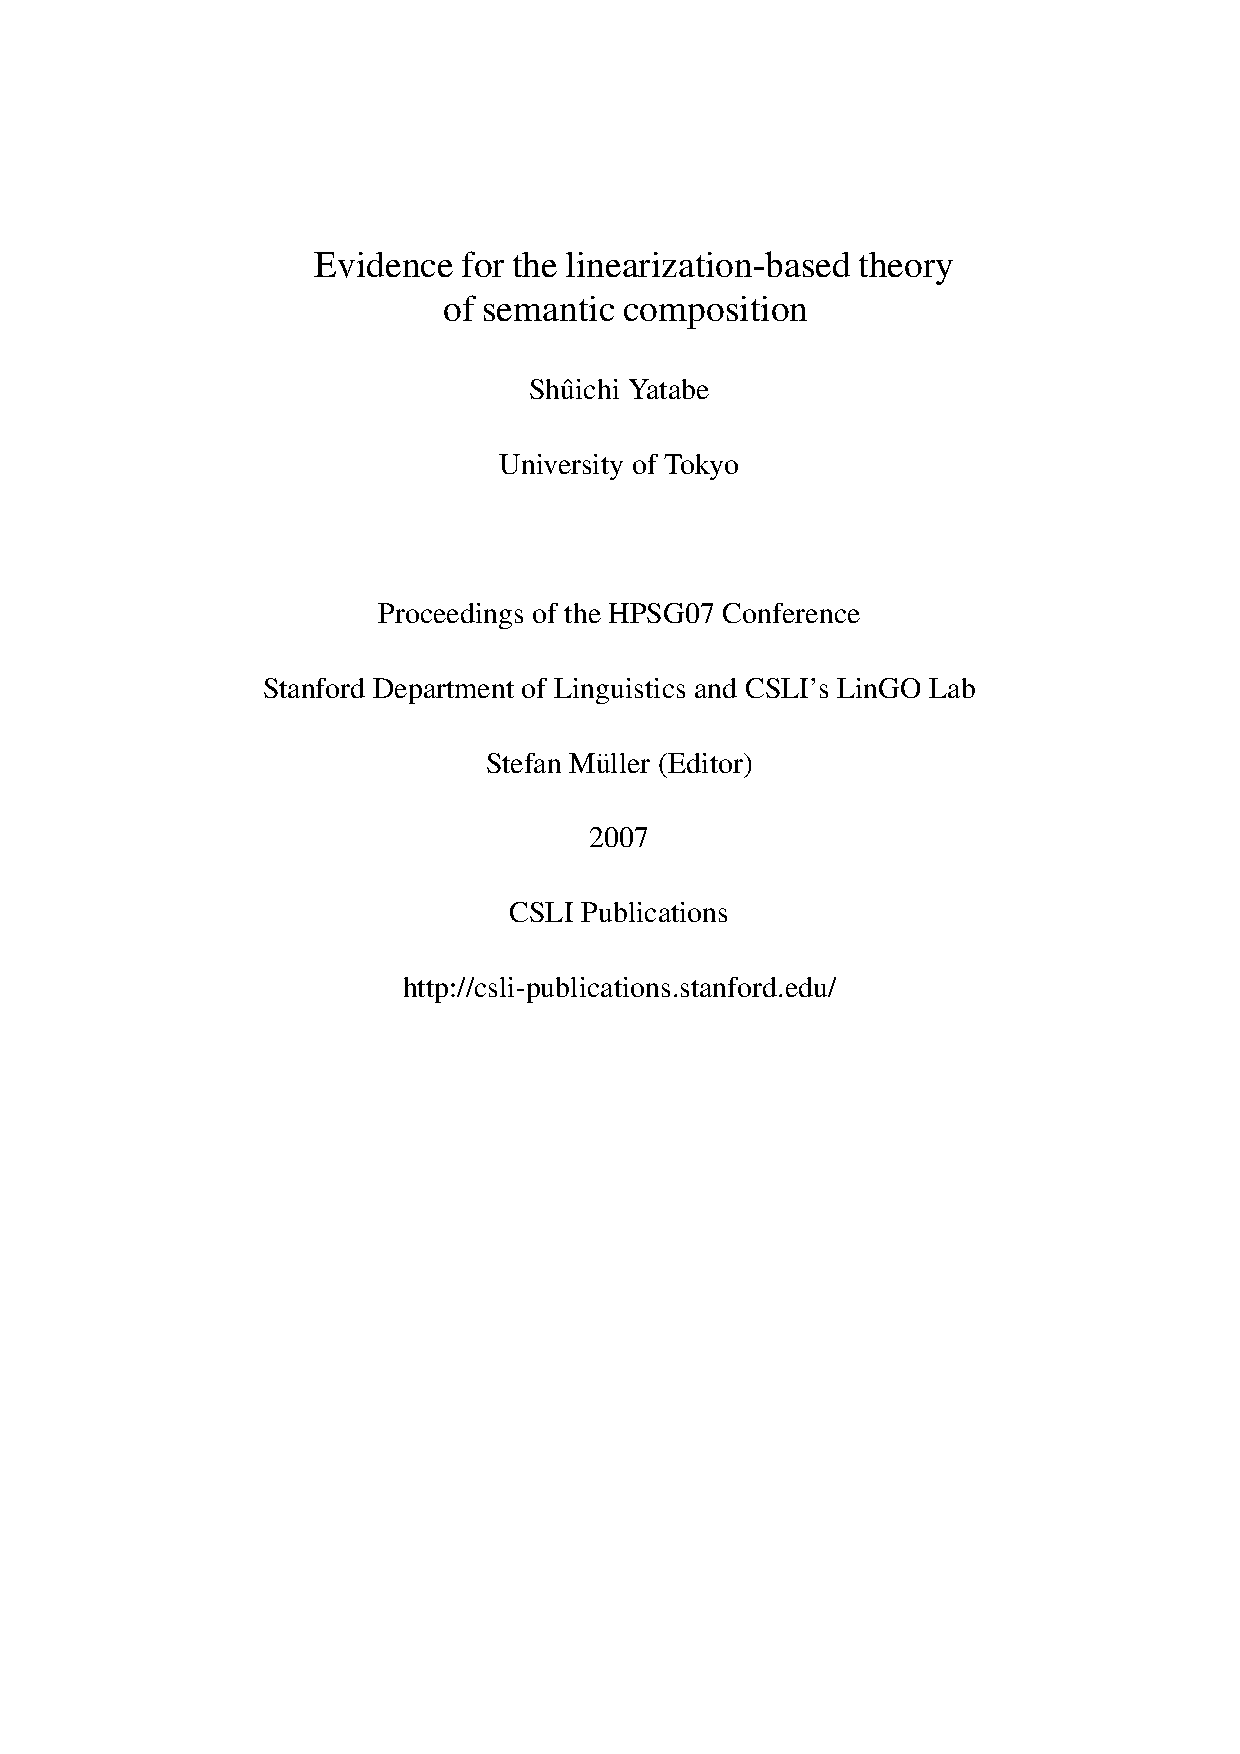
\includepdf[pages=-,pagecommand=\thispagestyle{plain},
            addtotoc={1,section,1,
            {Sh{\^{u}}ichi Yatabe: Evidence for the Linearization-Based Theory of Semantic Composition},
             yatabe}]{yatabe.pdf}

\newpage
\part{Contributions to the Workshop on \emph{Constructions and Grammatical Theory}}



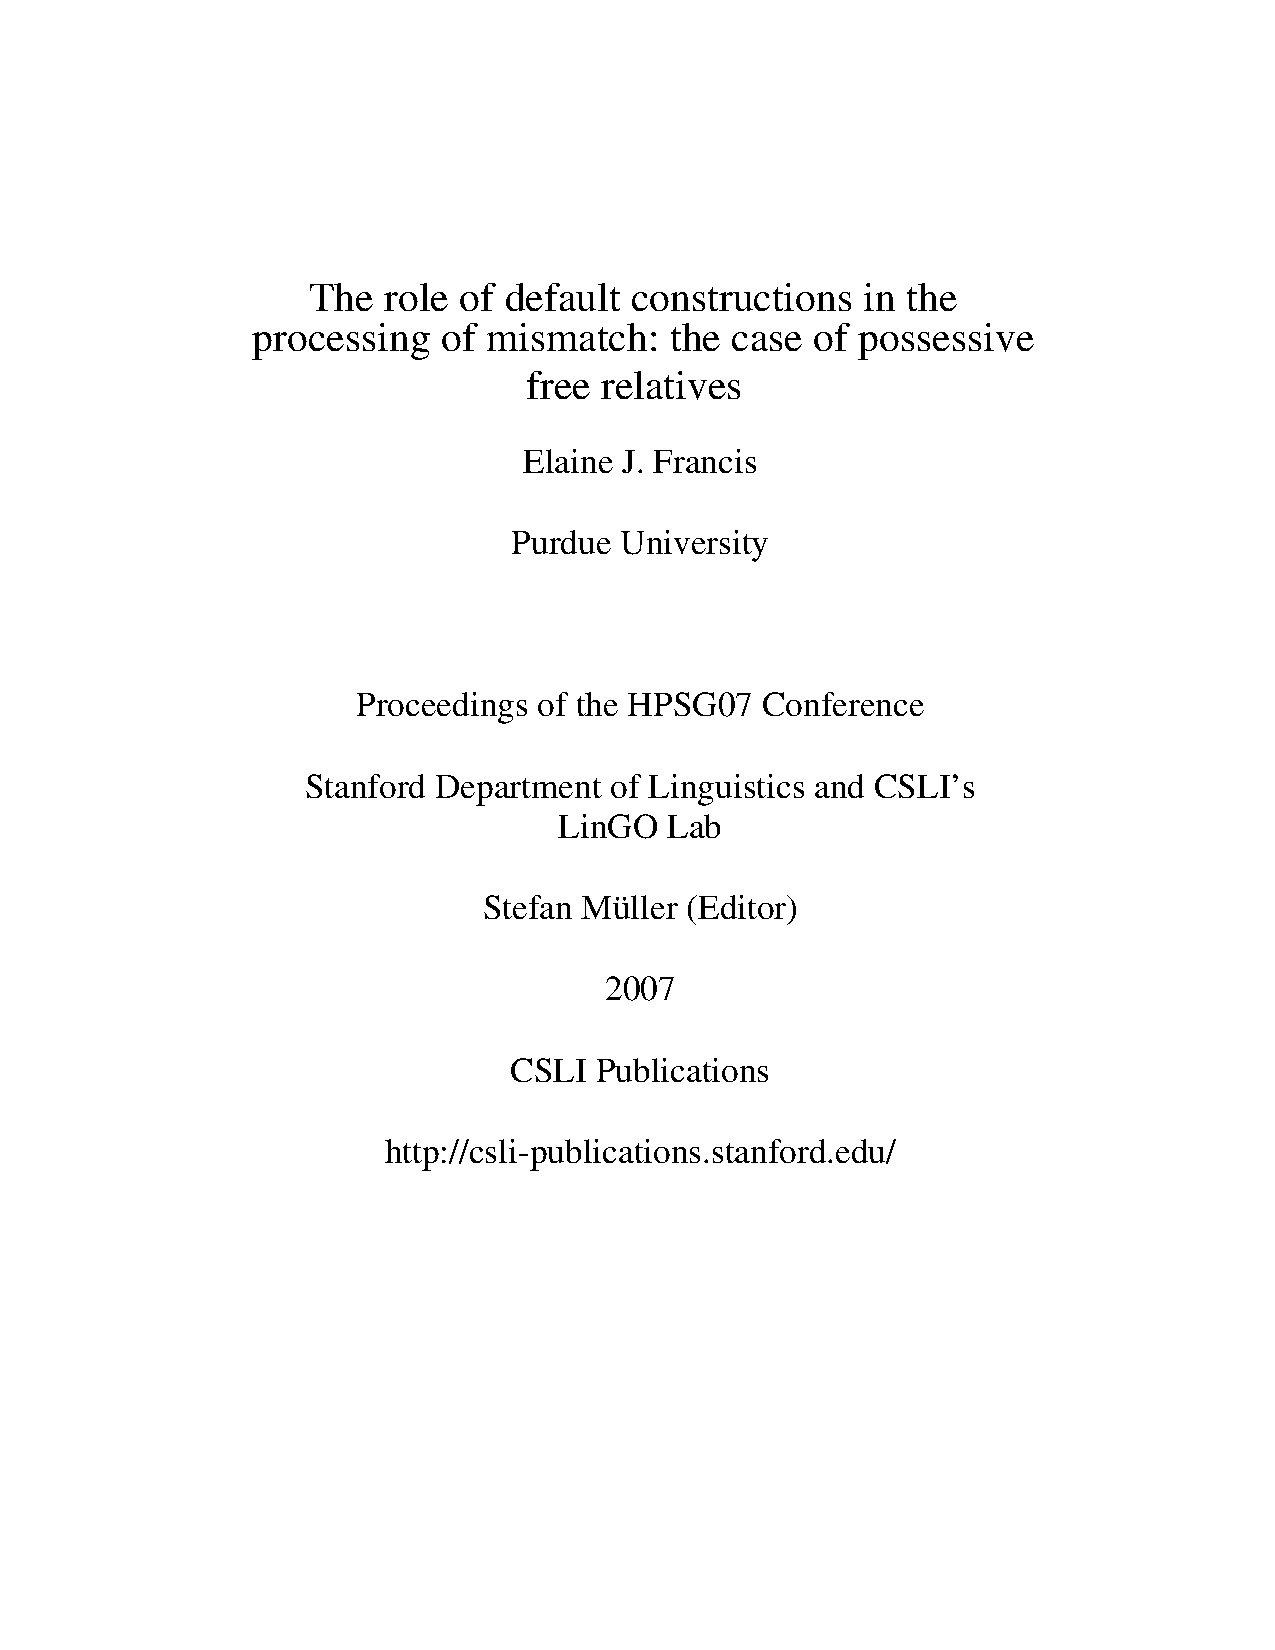
\includepdf[pages=-,pagecommand=\thispagestyle{plain},
            addtotoc={1,section,1,
            {Elaine J. Francis: The Role of Default Constructions in the Processing of Mismatch: the Case of Possessive Free Relatives},
             francis}]{francis.pdf}

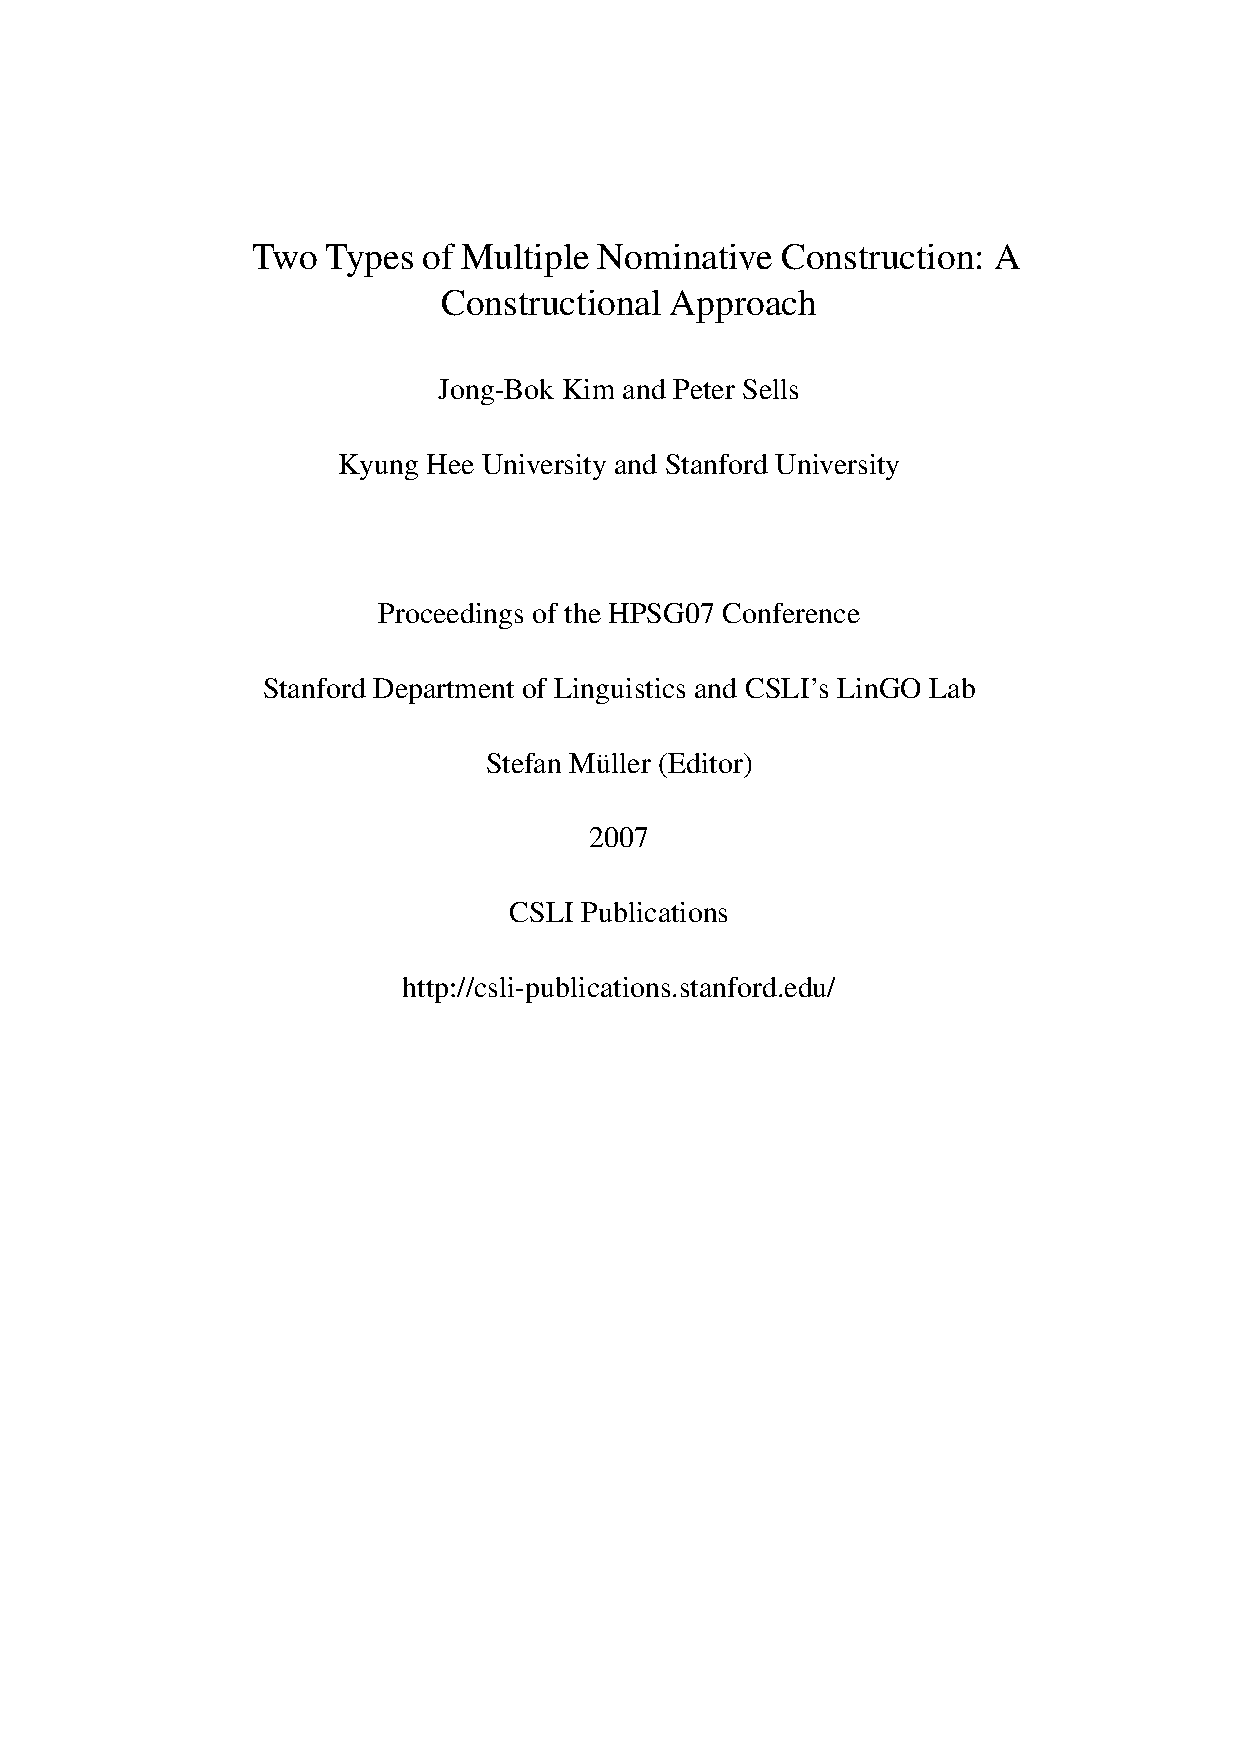
\includepdf[pages=-,pagecommand=\thispagestyle{plain},
            addtotoc={1,section,1,
            {Jong-Bok Kim and Peter Sells: Two Types of Multiple Nominative Construction: A Constructional Approach},
             ks}]{kim-sells.pdf}

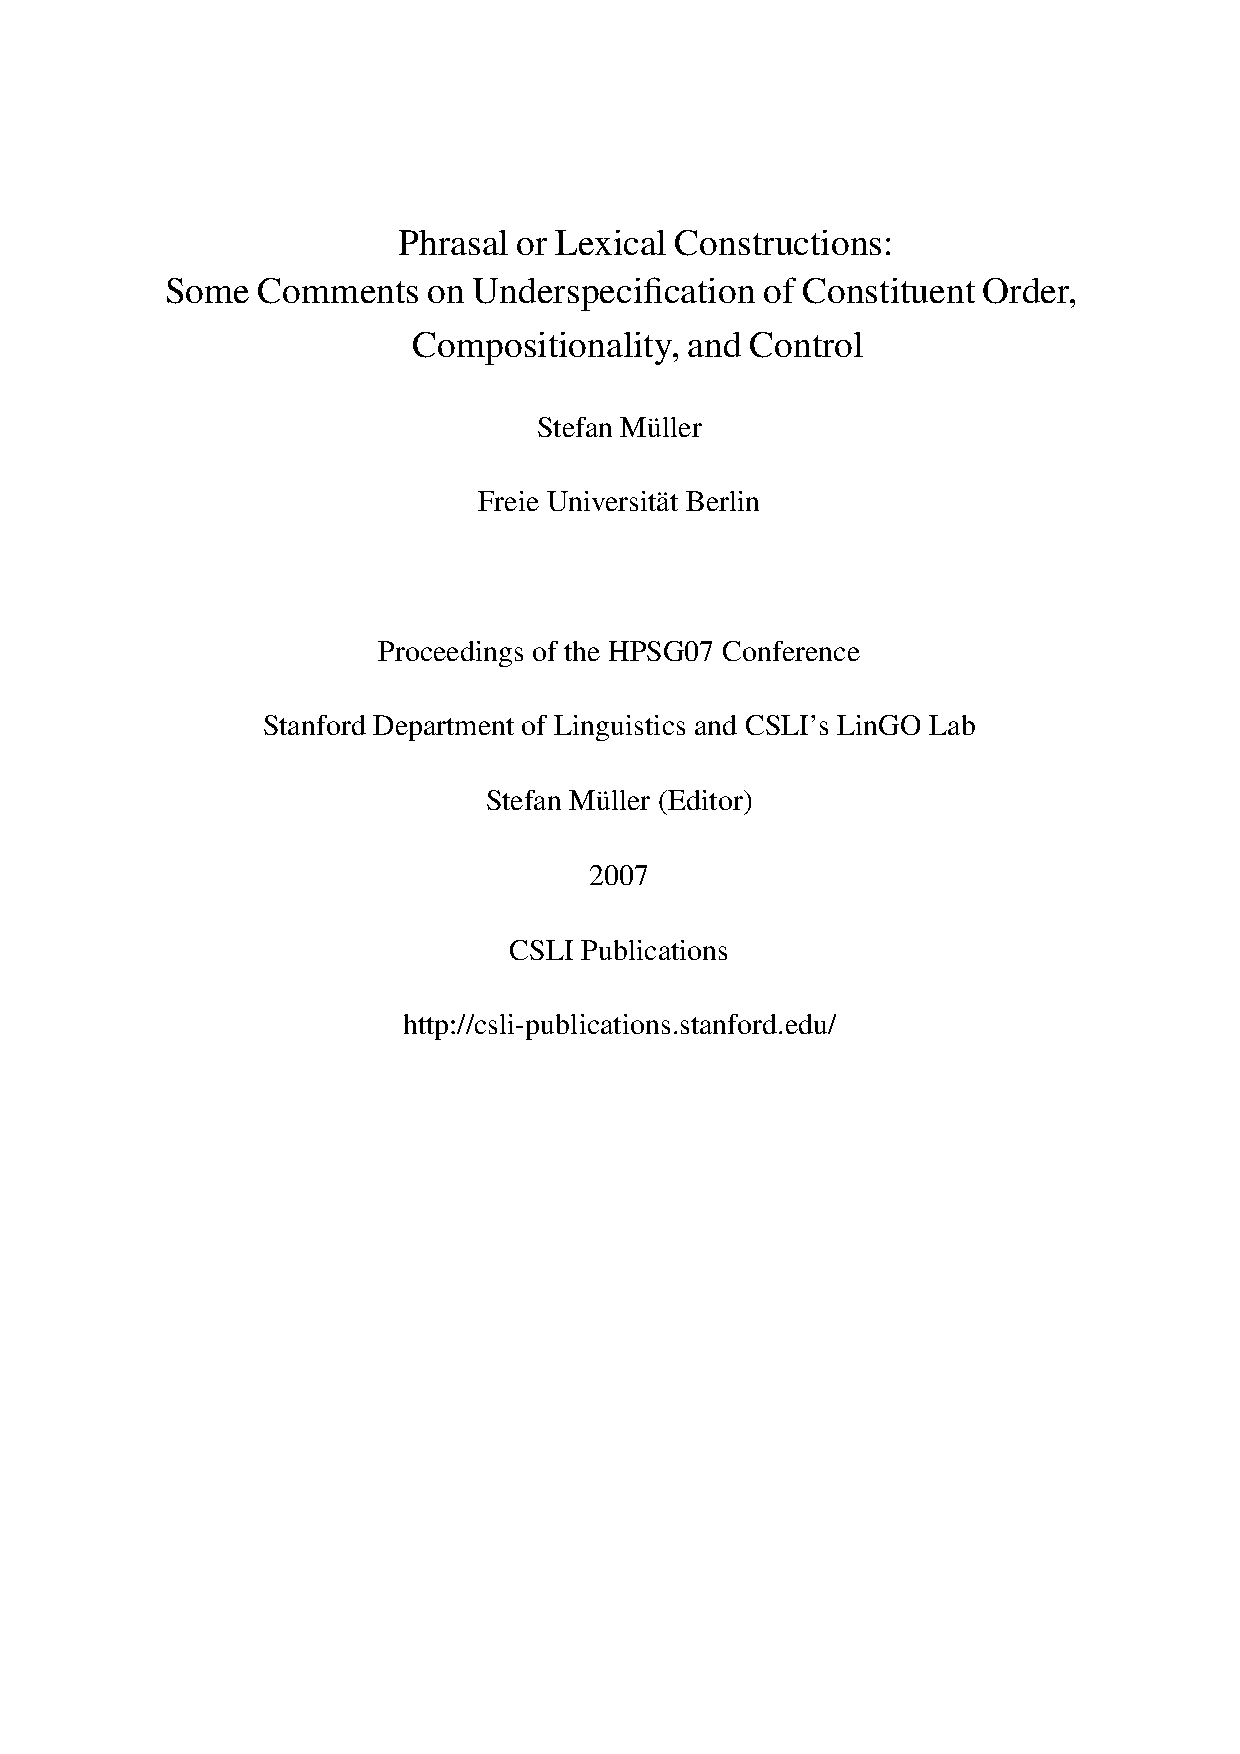
\includepdf[pages=-,pagecommand=\thispagestyle{plain},
            addtotoc={1,section,1,
            {Stefan M�ller: Phrasal or Lexical Constructions? Some Comments on Underspecification of Constituent
            Order, Compositionality, and Control},
             mueller}]{mueller.pdf}

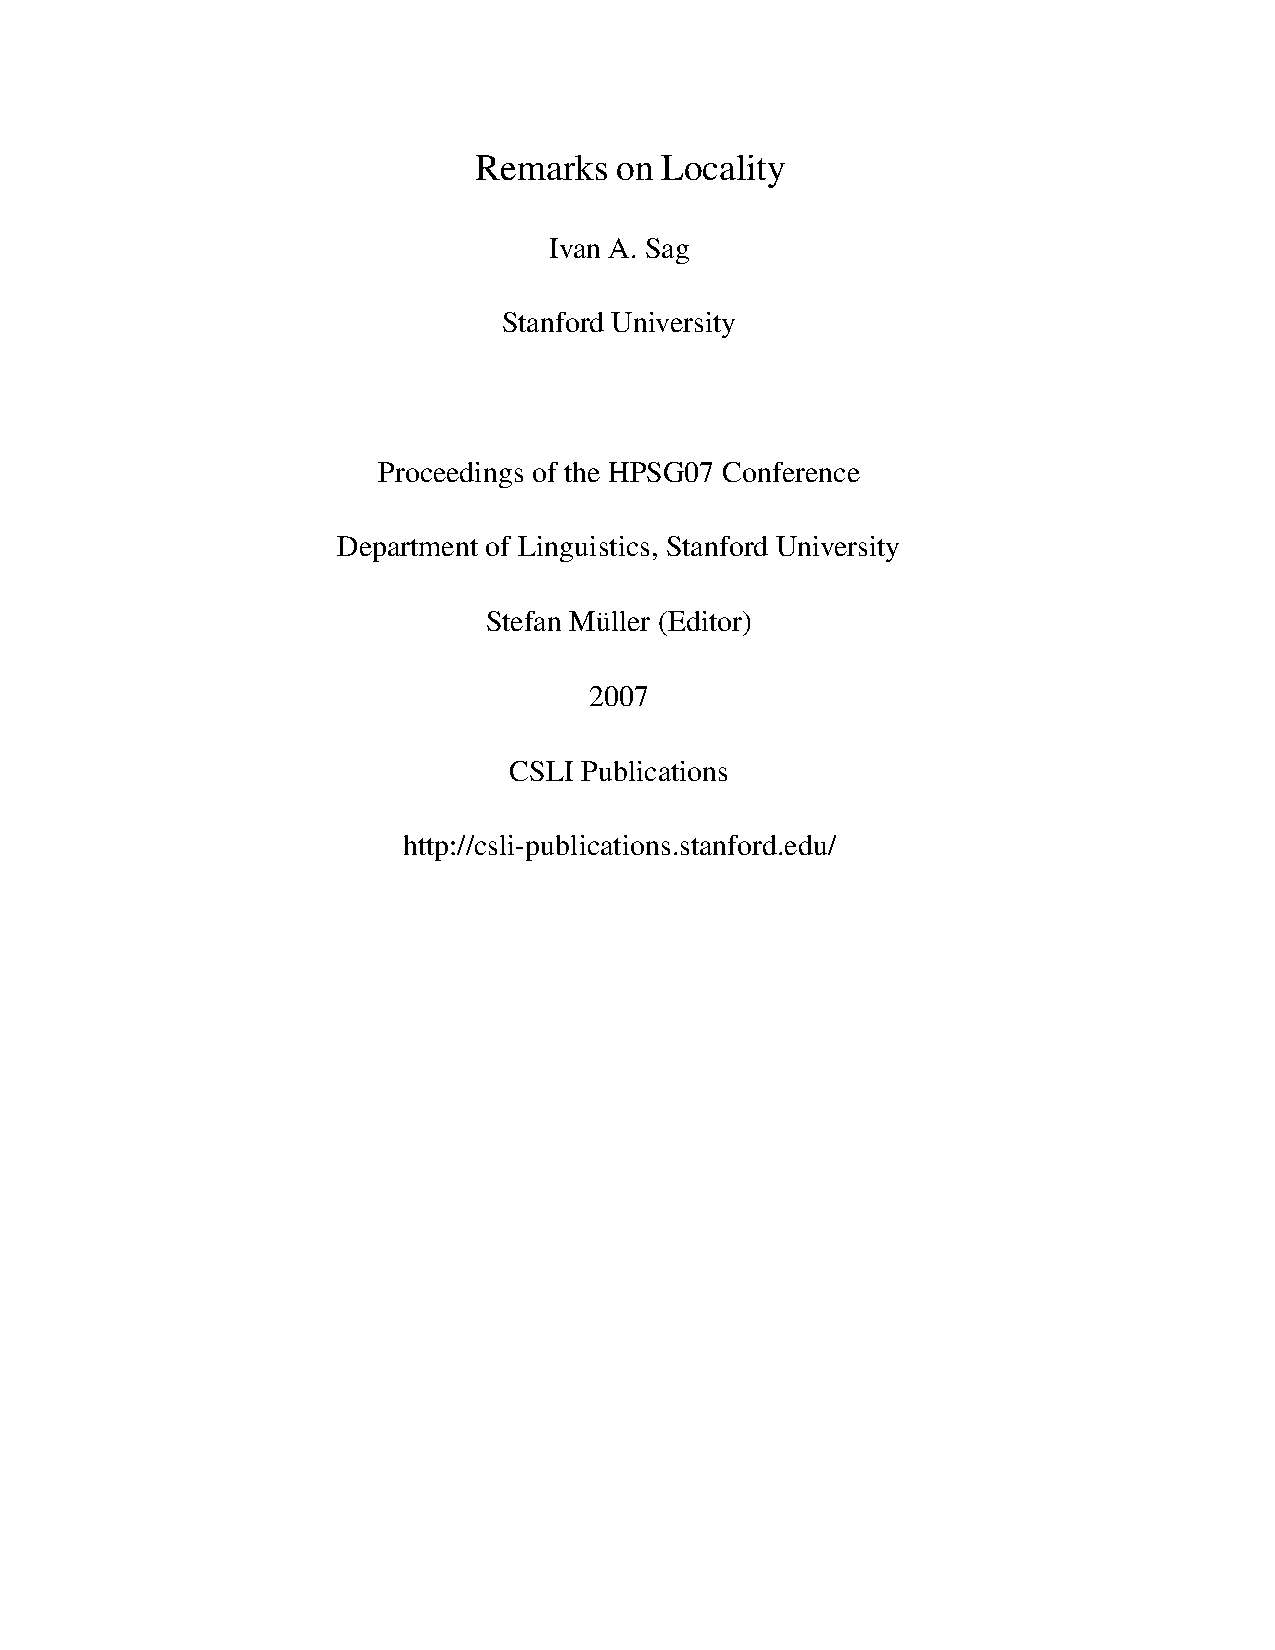
\includepdf[pages=-,pagecommand=\thispagestyle{plain},
            addtotoc={1,section,1,
            {Ivan A. Sag: Remarks on Locality},
             sag}]{sag.pdf}

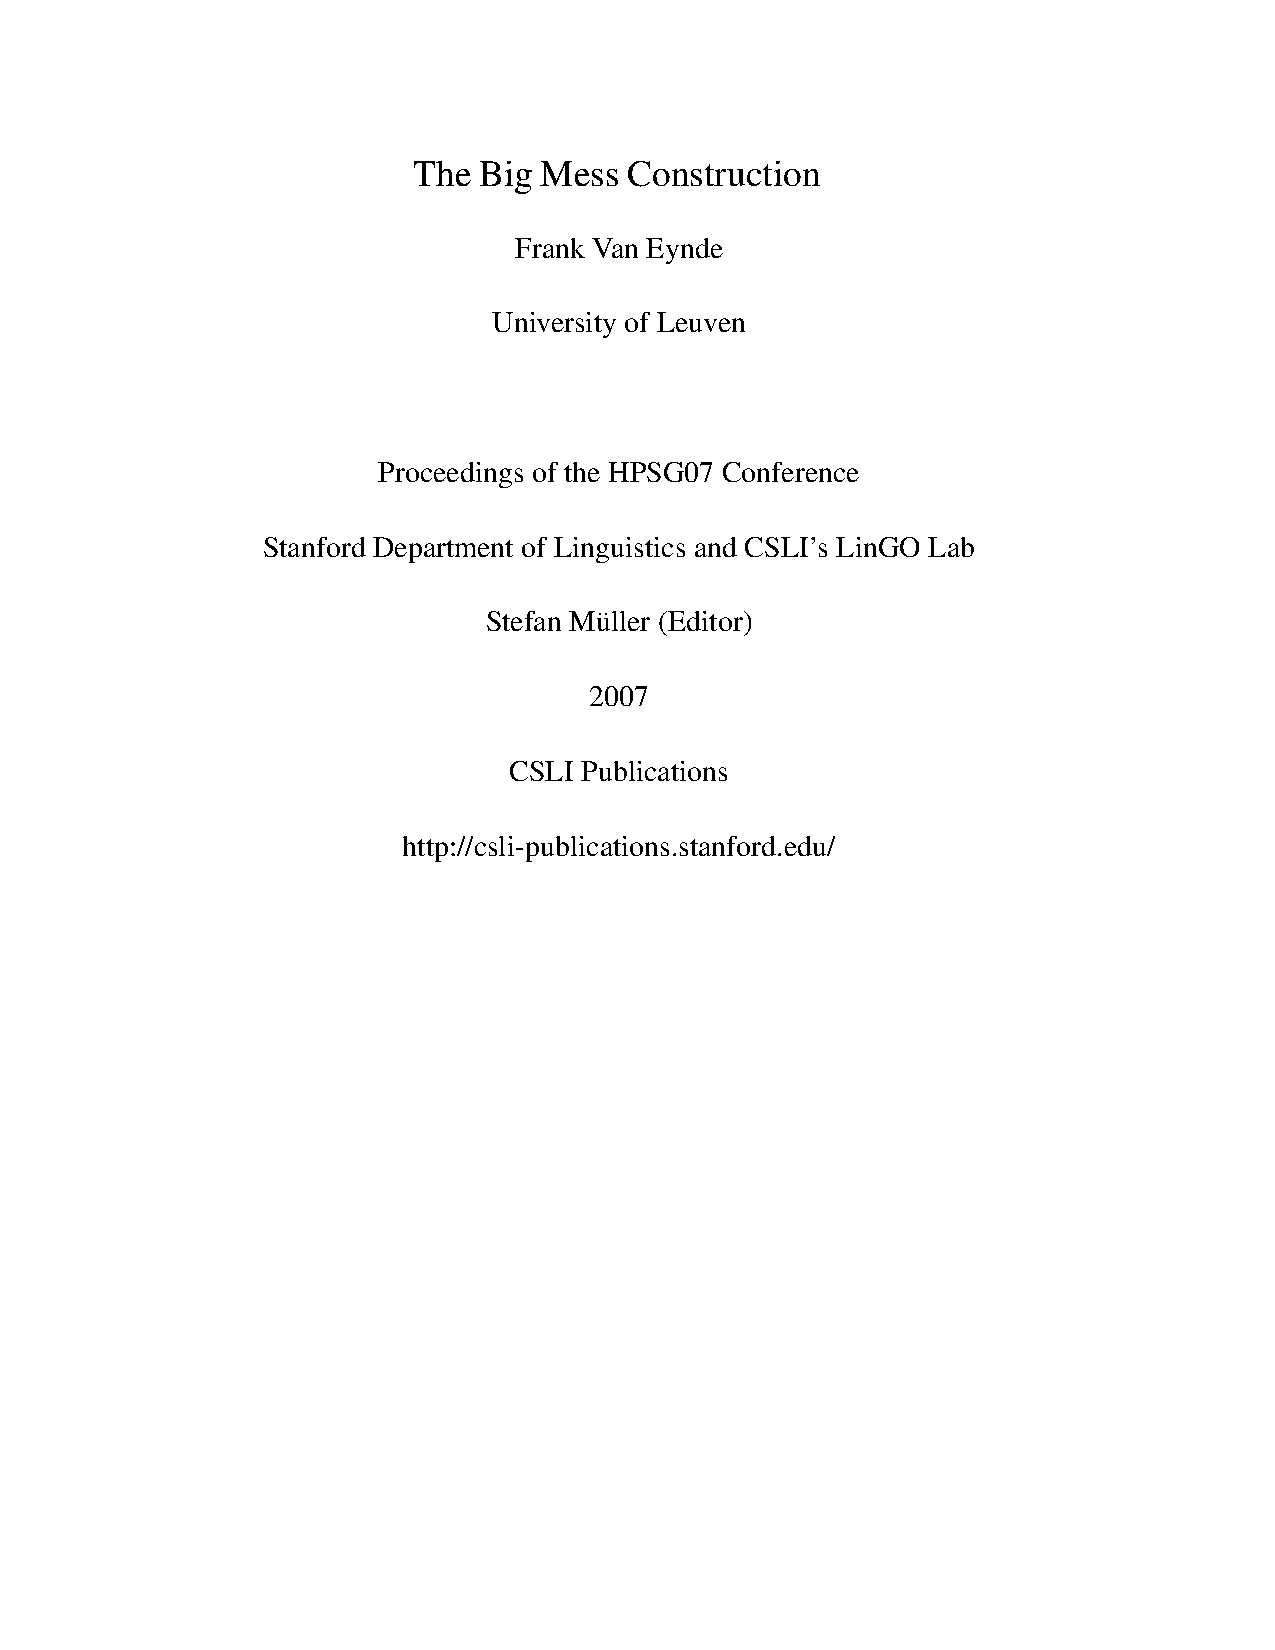
\includepdf[pages=-,pagecommand=\thispagestyle{plain},
            addtotoc={1,section,1,
            {Frank Van Eynde: The Big Mess Construction},
             vaneynde}]{vaneynde.pdf}





\end{document}

